% Options for packages loaded elsewhere
\PassOptionsToPackage{unicode}{hyperref}
\PassOptionsToPackage{hyphens}{url}
%
\documentclass[
]{article}
\usepackage{amsmath,amssymb}
\usepackage{lmodern}
\usepackage{ifxetex,ifluatex}
\ifnum 0\ifxetex 1\fi\ifluatex 1\fi=0 % if pdftex
  \usepackage[T1]{fontenc}
  \usepackage[utf8]{inputenc}
  \usepackage{textcomp} % provide euro and other symbols
\else % if luatex or xetex
  \usepackage{unicode-math}
  \defaultfontfeatures{Scale=MatchLowercase}
  \defaultfontfeatures[\rmfamily]{Ligatures=TeX,Scale=1}
\fi
% Use upquote if available, for straight quotes in verbatim environments
\IfFileExists{upquote.sty}{\usepackage{upquote}}{}
\IfFileExists{microtype.sty}{% use microtype if available
  \usepackage[]{microtype}
  \UseMicrotypeSet[protrusion]{basicmath} % disable protrusion for tt fonts
}{}
\makeatletter
\@ifundefined{KOMAClassName}{% if non-KOMA class
  \IfFileExists{parskip.sty}{%
    \usepackage{parskip}
  }{% else
    \setlength{\parindent}{0pt}
    \setlength{\parskip}{6pt plus 2pt minus 1pt}}
}{% if KOMA class
  \KOMAoptions{parskip=half}}
\makeatother
\usepackage{xcolor}
\IfFileExists{xurl.sty}{\usepackage{xurl}}{} % add URL line breaks if available
\IfFileExists{bookmark.sty}{\usepackage{bookmark}}{\usepackage{hyperref}}
\hypersetup{
  pdftitle={Chapter 4},
  pdfauthor={Randy},
  hidelinks,
  pdfcreator={LaTeX via pandoc}}
\urlstyle{same} % disable monospaced font for URLs
\usepackage[margin=1in]{geometry}
\usepackage{color}
\usepackage{fancyvrb}
\newcommand{\VerbBar}{|}
\newcommand{\VERB}{\Verb[commandchars=\\\{\}]}
\DefineVerbatimEnvironment{Highlighting}{Verbatim}{commandchars=\\\{\}}
% Add ',fontsize=\small' for more characters per line
\usepackage{framed}
\definecolor{shadecolor}{RGB}{248,248,248}
\newenvironment{Shaded}{\begin{snugshade}}{\end{snugshade}}
\newcommand{\AlertTok}[1]{\textcolor[rgb]{0.94,0.16,0.16}{#1}}
\newcommand{\AnnotationTok}[1]{\textcolor[rgb]{0.56,0.35,0.01}{\textbf{\textit{#1}}}}
\newcommand{\AttributeTok}[1]{\textcolor[rgb]{0.77,0.63,0.00}{#1}}
\newcommand{\BaseNTok}[1]{\textcolor[rgb]{0.00,0.00,0.81}{#1}}
\newcommand{\BuiltInTok}[1]{#1}
\newcommand{\CharTok}[1]{\textcolor[rgb]{0.31,0.60,0.02}{#1}}
\newcommand{\CommentTok}[1]{\textcolor[rgb]{0.56,0.35,0.01}{\textit{#1}}}
\newcommand{\CommentVarTok}[1]{\textcolor[rgb]{0.56,0.35,0.01}{\textbf{\textit{#1}}}}
\newcommand{\ConstantTok}[1]{\textcolor[rgb]{0.00,0.00,0.00}{#1}}
\newcommand{\ControlFlowTok}[1]{\textcolor[rgb]{0.13,0.29,0.53}{\textbf{#1}}}
\newcommand{\DataTypeTok}[1]{\textcolor[rgb]{0.13,0.29,0.53}{#1}}
\newcommand{\DecValTok}[1]{\textcolor[rgb]{0.00,0.00,0.81}{#1}}
\newcommand{\DocumentationTok}[1]{\textcolor[rgb]{0.56,0.35,0.01}{\textbf{\textit{#1}}}}
\newcommand{\ErrorTok}[1]{\textcolor[rgb]{0.64,0.00,0.00}{\textbf{#1}}}
\newcommand{\ExtensionTok}[1]{#1}
\newcommand{\FloatTok}[1]{\textcolor[rgb]{0.00,0.00,0.81}{#1}}
\newcommand{\FunctionTok}[1]{\textcolor[rgb]{0.00,0.00,0.00}{#1}}
\newcommand{\ImportTok}[1]{#1}
\newcommand{\InformationTok}[1]{\textcolor[rgb]{0.56,0.35,0.01}{\textbf{\textit{#1}}}}
\newcommand{\KeywordTok}[1]{\textcolor[rgb]{0.13,0.29,0.53}{\textbf{#1}}}
\newcommand{\NormalTok}[1]{#1}
\newcommand{\OperatorTok}[1]{\textcolor[rgb]{0.81,0.36,0.00}{\textbf{#1}}}
\newcommand{\OtherTok}[1]{\textcolor[rgb]{0.56,0.35,0.01}{#1}}
\newcommand{\PreprocessorTok}[1]{\textcolor[rgb]{0.56,0.35,0.01}{\textit{#1}}}
\newcommand{\RegionMarkerTok}[1]{#1}
\newcommand{\SpecialCharTok}[1]{\textcolor[rgb]{0.00,0.00,0.00}{#1}}
\newcommand{\SpecialStringTok}[1]{\textcolor[rgb]{0.31,0.60,0.02}{#1}}
\newcommand{\StringTok}[1]{\textcolor[rgb]{0.31,0.60,0.02}{#1}}
\newcommand{\VariableTok}[1]{\textcolor[rgb]{0.00,0.00,0.00}{#1}}
\newcommand{\VerbatimStringTok}[1]{\textcolor[rgb]{0.31,0.60,0.02}{#1}}
\newcommand{\WarningTok}[1]{\textcolor[rgb]{0.56,0.35,0.01}{\textbf{\textit{#1}}}}
\usepackage{graphicx}
\makeatletter
\def\maxwidth{\ifdim\Gin@nat@width>\linewidth\linewidth\else\Gin@nat@width\fi}
\def\maxheight{\ifdim\Gin@nat@height>\textheight\textheight\else\Gin@nat@height\fi}
\makeatother
% Scale images if necessary, so that they will not overflow the page
% margins by default, and it is still possible to overwrite the defaults
% using explicit options in \includegraphics[width, height, ...]{}
\setkeys{Gin}{width=\maxwidth,height=\maxheight,keepaspectratio}
% Set default figure placement to htbp
\makeatletter
\def\fps@figure{htbp}
\makeatother
\setlength{\emergencystretch}{3em} % prevent overfull lines
\providecommand{\tightlist}{%
  \setlength{\itemsep}{0pt}\setlength{\parskip}{0pt}}
\setcounter{secnumdepth}{-\maxdimen} % remove section numbering
\ifluatex
  \usepackage{selnolig}  % disable illegal ligatures
\fi

\title{Chapter 4}
\author{Randy}
\date{7/10/2021}

\begin{document}
\maketitle

\hypertarget{covariance-functions}{%
\section{Covariance Functions}\label{covariance-functions}}

\begin{itemize}
\tightlist
\item
  similarity
\item
  covariance function
\end{itemize}

\hypertarget{preliminaries}{%
\subsection{4.1 Preliminaries}\label{preliminaries}}

\begin{itemize}
\item
  stationary
\item
  isotropy
\item
  dot product covariance
\item
  kernel
\item
  Gram matrix
\item
  covariance matrix
\item
  positive semi-definite
\end{itemize}

\[
(T_kf)(x) = \int_{\mathcal{X}} k(x,\ x')f(x')d\mu(x') \ \ \ (4.1)
\]

\[
Q(v)\ =\ v^{\top}Kv\ \geq 0,\ \forall v \in \mathbb{R}^n\\
\int k(x, x')f(x)f(x') dµ(x) dµ(x') \geq 0,\ \forall f \in L_2(\mathcal{X}, \mu) \ \ \ (4.2)
\]

\[
\mathbb {E}[N_u] = \frac{1} {2\pi}\sqrt{\frac{-k''(0)}{k(0)}}exp\Big(-\frac{u^2}{2k(0)}\Big) \ \ \ (4.3)
\]

\hypertarget{mean-square-continuity-and-differentiability}{%
\subsubsection{4.1.1 Mean Square Continuity and
Differentiability}\label{mean-square-continuity-and-differentiability}}

\begin{itemize}
\item
  Let \(\pmb x_1\), \(\pmb x_2\), \ldots{} be a sequence of points and
  \(x_*\) be a fixed point in \(\mathbb R^D\) such that
  \(|\pmb x_k - \pmb x_*| \rightarrow 0\) as \(k \rightarrow \infty\).
  Then a process \(f(\pmb x)\) is continuous in mean square at
  \(\pmb x_*\) if \(E[|f(\pmb x_k) - f(\pmb x_*)|^2] \rightarrow 0\) as
  mean square continuity as \(k \rightarrow \infty\).
\item
  If this holds for all \(x_* \in \mathcal A\) where \(\mathcal A\) is a
  subset of \(\mathbb R^D\) then \(f(\pmb x)\) is said to be continuous
  in mean square (MS) over \(\mathcal A\).
\item
  A random field is continuous in mean square at \(x^*\) if and only if
  its covariance function \(k(x, x')\) is continuous at the point
  \(x = x' = x^*\)
\item
  For stationary covariance functions this reduces to checking
  continuity at \(k(\pmb 0)\). Note that MS continuity does not
  necessarily imply sample function continuity
\end{itemize}

\[
\frac {\partial f(\pmb x)}
{\partial x_i} = \lim_ {h \rightarrow 0} 
\frac {f(\pmb x + h \pmb e_i) - f(\pmb x)} {h}
\ \ \ \ (4.4)
\]

Notice that it is the properties of the kernel \(k\) around \(\pmb 0\)
that determine the smoothness properties (MS differentiability) of a
stationary process.

\hypertarget{examples-of-covariance-functions}{%
\subsection{4.2 Examples of Covariance
Functions}\label{examples-of-covariance-functions}}

\hypertarget{stationary-covariance-functions}{%
\subsubsection{4.2.1 Stationary Covariance
Functions}\label{stationary-covariance-functions}}

\hypertarget{theorem-4.1-bochners-theorem}{%
\paragraph{Theorem 4.1 (Bochner's
theorem)}\label{theorem-4.1-bochners-theorem}}

A complex-valued function \(k\) on \(\mathbb R^D\) is the covariance
function of a weakly stationary mean square continuous complex valued
random process on \(\mathbb R^D\) if and only if it can be represented
as

\[
k(\tau) = \int_{\mathbb{R}^D} e^{2\pi i \pmb{s} \cdot \pmb{\tau}} d\mu (s) \ \ \ (4.5)
\]

where \(\mu\) is a positive finite measure

\hypertarget{wiener-khintchine-theorem}{%
\paragraph{Wiener-Khintchine theorem}\label{wiener-khintchine-theorem}}

The covariance function and the spectral density are Fourier duals

\[
k(\tau) = \int S(s) e^{2\pi is \cdot \tau} ds
\ \ \ \ (4.6a)\\
S(s) = \int k(\tau) e^{-2\pi is\cdot \tau} d\tau
\ \ \ \ (4.6b)\\
k(\pmb 0) = \int S(s)ds
\]

use spherical polar coordinates and integrating out the angular
variables

\[
{S(\pmb s):\ s \stackrel {\Delta}{=} |\pmb s|}\\
k(r) = \frac {2\pi} {r^{D/2-1}} 
\int _0^{\infty} S(s)J_{D/2-1}
(2\pi rs)s^{D/2} ds \ \ \  (4.7)\\
S(s) = \frac {2\pi} {s^{D/2-1}} 
\int _0^{\infty} k(r)J_{D/2-1}
(2\pi rs) r^{D/2} dr\ \ \ \ (4.8)
\]

\hypertarget{squared-exponential-covariance-function}{%
\paragraph{Squared Exponential Covariance
Function}\label{squared-exponential-covariance-function}}

\[
k_{SE}(r) = exp \Big(- \frac {r^2} {2l^2} \Big) 
\ \ \ \ (4.9a)\\
S(s) = (2\pi l^2)^{D/2} exp(-2\pi^2l^2s^2)
\ \ \ \ (4.9b)
\]

\[
\phi_c(x) = exp \Big(- \frac {(x - c)^2} {2l^2}\Big)
\ \ \ \ (4.10)
\]

\[
k(x_p, x_q) = \sigma_p^2\sum_{c=1}{N}
\phi_c(x_p)\phi_c(x_q)
\ \ \ \ (4.11)
\]

\[
\lim_{N \rightarrow \infty}
\frac {\sigma^2_p} N \sum _{c=1}^N 
\phi_c(x_p)\phi_c(x_q) = \sigma_p^2 
\int ^{c_{max}}_{c_{min}} 
\phi_c(x_p)\phi_c(x_q)dc
\ \ \ \ (4.12)
\]

\[
k(x_p, x_q) = \sigma_p^2 \int_{-\infty}^{\infty} 
exp \Big(- \frac {(x_p - c)^2} {2l^2}\Big)
exp \Big(- \frac {(x_q - c)^2} {2l^2}\Big) dc\\
= \sqrt {\pi} l \sigma_p^2 
exp \Bigg(- \frac {(x_p - x_q)^2} {2(\sqrt 2l)^2} \Bigg)
\ \ \ \ (4.13)
\]

\begin{Shaded}
\begin{Highlighting}[]
\NormalTok{get\_symm }\OtherTok{\textless{}{-}} \ControlFlowTok{function}\NormalTok{(M) \{}
\NormalTok{   M[}\FunctionTok{upper.tri}\NormalTok{(M)] }\OtherTok{\textless{}{-}} \FunctionTok{t}\NormalTok{(M)[}\FunctionTok{upper.tri}\NormalTok{(M)]}
   \FunctionTok{return}\NormalTok{(M)}
\NormalTok{\}}
\end{Highlighting}
\end{Shaded}

\begin{Shaded}
\begin{Highlighting}[]
\FunctionTok{set.seed}\NormalTok{(}\DecValTok{55}\NormalTok{)}
\DocumentationTok{\#\# for one squared exponential kernel {-}{-}{-}{-}{-}{-}{-}{-}{-}{-}{-}{-}{-}{-}{-}{-}{-}{-}{-}{-}{-}{-}{-}{-}{-}{-}{-}{-}{-}{-}{-}{-}{-}{-}{-}{-}{-}{-}{-}{-}{-}{-}{-}{-}{-}}
\DocumentationTok{\#\# simulate 100 points}
\NormalTok{x }\OtherTok{\textless{}{-}} \FunctionTok{runif}\NormalTok{(}\DecValTok{100}\NormalTok{)}
\DocumentationTok{\#\# compute distance matrix}
\NormalTok{d }\OtherTok{\textless{}{-}} \FunctionTok{abs}\NormalTok{(}\FunctionTok{outer}\NormalTok{(x, x, }\AttributeTok{FUN =} \StringTok{"{-}"}\NormalTok{))}
\DocumentationTok{\#\# the characteristic length scale}
\NormalTok{l0 }\OtherTok{\textless{}{-}} \DecValTok{1}
\CommentTok{\# squared exponential kernel}
\NormalTok{kernel\_se }\OtherTok{\textless{}{-}} \FunctionTok{exp}\NormalTok{(}\SpecialCharTok{{-}}\NormalTok{d}\SpecialCharTok{\^{}}\DecValTok{2} \SpecialCharTok{/}\NormalTok{ (}\DecValTok{2} \SpecialCharTok{*}\NormalTok{ l0}\SpecialCharTok{\^{}}\DecValTok{2}\NormalTok{)) }
\NormalTok{sim }\OtherTok{\textless{}{-}}\NormalTok{ mvtnorm}\SpecialCharTok{::}\FunctionTok{rmvnorm}\NormalTok{(}\DecValTok{5}\NormalTok{, }\AttributeTok{sigma =}\NormalTok{ kernel\_se)}
\NormalTok{data }\OtherTok{\textless{}{-}} \FunctionTok{cbind}\NormalTok{(x, }\FunctionTok{t}\NormalTok{(sim)) }\SpecialCharTok{\%\textgreater{}\%} 
    \FunctionTok{data.frame}\NormalTok{() }\SpecialCharTok{\%\textgreater{}\%}
    \FunctionTok{arrange}\NormalTok{(}\AttributeTok{by =}\NormalTok{ x)}
\FunctionTok{matplot}\NormalTok{(data[, }\DecValTok{1}\NormalTok{], data[, }\SpecialCharTok{{-}}\DecValTok{1}\NormalTok{], }\StringTok{"l"}\NormalTok{, }
        \AttributeTok{xlab =} \StringTok{"input, x"}\NormalTok{, }\AttributeTok{ylab =} \StringTok{"output, y"}\NormalTok{, }
        \AttributeTok{ylim =} \FunctionTok{c}\NormalTok{(}\SpecialCharTok{{-}}\DecValTok{2}\NormalTok{, }\DecValTok{2}\NormalTok{))}
\end{Highlighting}
\end{Shaded}

\begin{center}\includegraphics[width=0.4\linewidth]{04_gaussian_ch4_files/figure-latex/unnamed-chunk-2-1} \end{center}

\begin{Shaded}
\begin{Highlighting}[]
\NormalTok{r }\OtherTok{=} \FunctionTok{seq}\NormalTok{(}\DecValTok{0}\NormalTok{, }\DecValTok{3}\NormalTok{, }\AttributeTok{len =} \DecValTok{100}\NormalTok{)}
\NormalTok{l1 }\OtherTok{\textless{}{-}} \FunctionTok{c}\NormalTok{(}\FloatTok{0.01}\NormalTok{, }\FloatTok{0.1}\NormalTok{,  }\FloatTok{0.5}\NormalTok{,}
         \FloatTok{0.9}\NormalTok{,   }\DecValTok{1}\NormalTok{,  }\FloatTok{1.2}\NormalTok{, }
           \DecValTok{2}\NormalTok{,   }\DecValTok{5}\NormalTok{,  }\DecValTok{10}\NormalTok{)}

\NormalTok{kernel\_se }\OtherTok{\textless{}{-}} \FunctionTok{matrix}\NormalTok{(}\AttributeTok{data =} \ConstantTok{NA}\NormalTok{, }\AttributeTok{nrow =} \FunctionTok{length}\NormalTok{(l1), }\AttributeTok{ncol =} \FunctionTok{length}\NormalTok{(r))}
\ControlFlowTok{for}\NormalTok{ (i }\ControlFlowTok{in} \DecValTok{1}\SpecialCharTok{:}\DecValTok{9}\NormalTok{) \{}
  \ControlFlowTok{for}\NormalTok{ (j }\ControlFlowTok{in} \DecValTok{1}\SpecialCharTok{:}\FunctionTok{length}\NormalTok{(r)) \{}
\NormalTok{    kernel\_se[i, j] }\OtherTok{\textless{}{-}} \FunctionTok{exp}\NormalTok{(}\SpecialCharTok{{-}}\NormalTok{r[j]}\SpecialCharTok{\^{}}\DecValTok{2} \SpecialCharTok{/}\NormalTok{ (}\DecValTok{2} \SpecialCharTok{*}\NormalTok{ l1[i]}\SpecialCharTok{\^{}}\DecValTok{2}\NormalTok{))}
\NormalTok{  \}}
\NormalTok{\}}
\FunctionTok{matplot}\NormalTok{(r, }\FunctionTok{t}\NormalTok{(kernel\_se), }
        \AttributeTok{xlab =} \StringTok{"input, x"}\NormalTok{, }\AttributeTok{ylab =} \StringTok{"output, y"}\NormalTok{,}
        \StringTok{"l"}\NormalTok{)}
\end{Highlighting}
\end{Shaded}

\begin{center}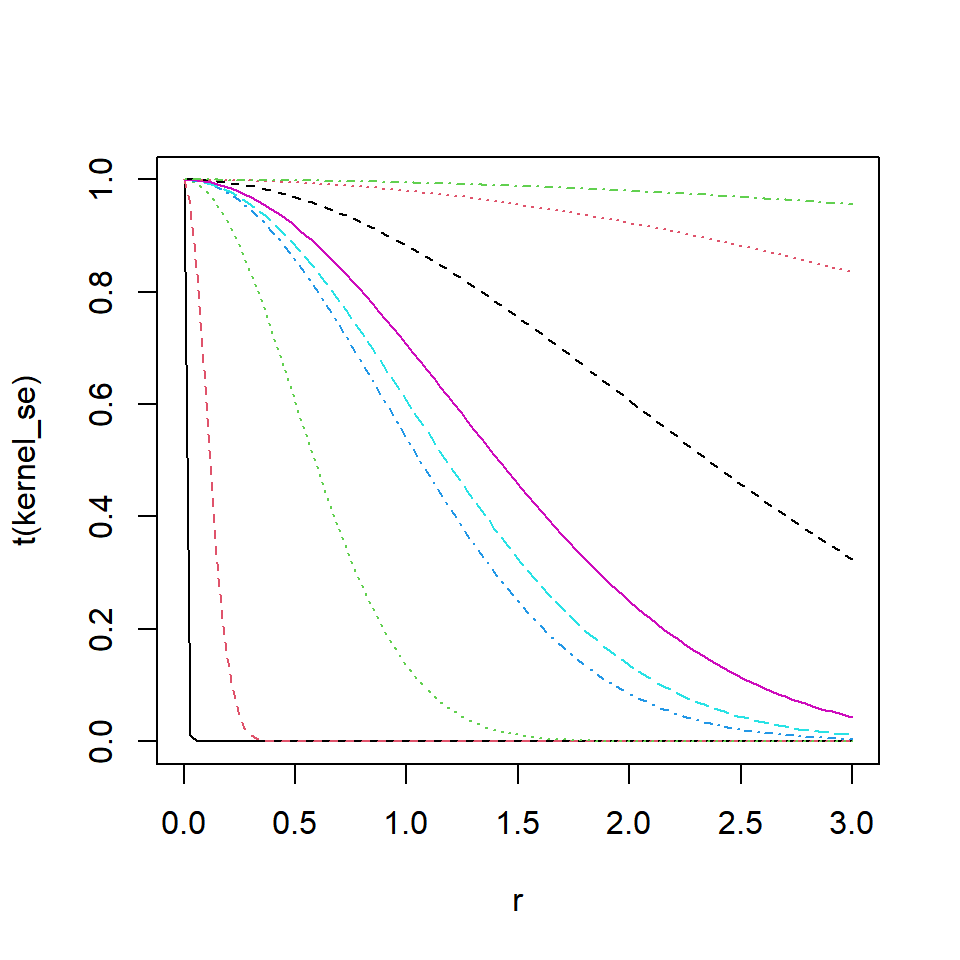
\includegraphics[width=0.4\linewidth]{04_gaussian_ch4_files/figure-latex/se kernel-1} \end{center}

\begin{Shaded}
\begin{Highlighting}[]
\DocumentationTok{\#\# change the characteristic length {-}{-}{-}{-}{-}{-}{-}{-}{-}{-}{-}{-}{-}{-}{-}{-}{-}{-}{-}{-}{-}{-}{-}{-}{-}{-}{-}{-}{-}{-}{-}{-}{-}{-}{-}{-}{-}{-}{-}{-}{-}{-}{-}{-}{-}}

\NormalTok{l1 }\OtherTok{\textless{}{-}} \FunctionTok{c}\NormalTok{(}\FloatTok{0.01}\NormalTok{, }\FloatTok{0.1}\NormalTok{,  }\FloatTok{0.5}\NormalTok{,}
         \FloatTok{0.9}\NormalTok{,   }\DecValTok{1}\NormalTok{,  }\FloatTok{1.2}\NormalTok{, }
           \DecValTok{2}\NormalTok{,   }\DecValTok{5}\NormalTok{,  }\DecValTok{10}\NormalTok{)}
\NormalTok{op }\OtherTok{\textless{}{-}} \FunctionTok{par}\NormalTok{(}\AttributeTok{mfrow =} \FunctionTok{c}\NormalTok{(}\DecValTok{3}\NormalTok{, }\DecValTok{3}\NormalTok{))}
\ControlFlowTok{for}\NormalTok{ (i }\ControlFlowTok{in} \DecValTok{1}\SpecialCharTok{:}\DecValTok{9}\NormalTok{) \{}
\NormalTok{  kernel\_se }\OtherTok{\textless{}{-}} \FunctionTok{exp}\NormalTok{(}\SpecialCharTok{{-}}\NormalTok{d}\SpecialCharTok{\^{}}\DecValTok{2} \SpecialCharTok{/}\NormalTok{ (}\DecValTok{2} \SpecialCharTok{*}\NormalTok{ l1[i]}\SpecialCharTok{\^{}}\DecValTok{2}\NormalTok{)) }
\NormalTok{  sim }\OtherTok{\textless{}{-}}\NormalTok{ mvtnorm}\SpecialCharTok{::}\FunctionTok{rmvnorm}\NormalTok{(}\DecValTok{5}\NormalTok{, }\AttributeTok{sigma =}\NormalTok{ kernel\_se)}
\NormalTok{  data }\OtherTok{\textless{}{-}} \FunctionTok{cbind}\NormalTok{(x, }\FunctionTok{t}\NormalTok{(sim)) }\SpecialCharTok{\%\textgreater{}\%} 
    \FunctionTok{data.frame}\NormalTok{() }\SpecialCharTok{\%\textgreater{}\%}
    \FunctionTok{arrange}\NormalTok{(}\AttributeTok{by =}\NormalTok{ x)}
  \FunctionTok{matplot}\NormalTok{(data[, }\DecValTok{1}\NormalTok{], data[, }\SpecialCharTok{{-}}\DecValTok{1}\NormalTok{], }
          \AttributeTok{xlab =} \StringTok{"input, x"}\NormalTok{, }\AttributeTok{ylab =} \StringTok{"output, y"}\NormalTok{,}
          \StringTok{"l"}\NormalTok{, }\AttributeTok{ylim =} \FunctionTok{c}\NormalTok{(}\SpecialCharTok{{-}}\DecValTok{2}\NormalTok{, }\DecValTok{2}\NormalTok{))}
\NormalTok{\}}
\end{Highlighting}
\end{Shaded}

\begin{center}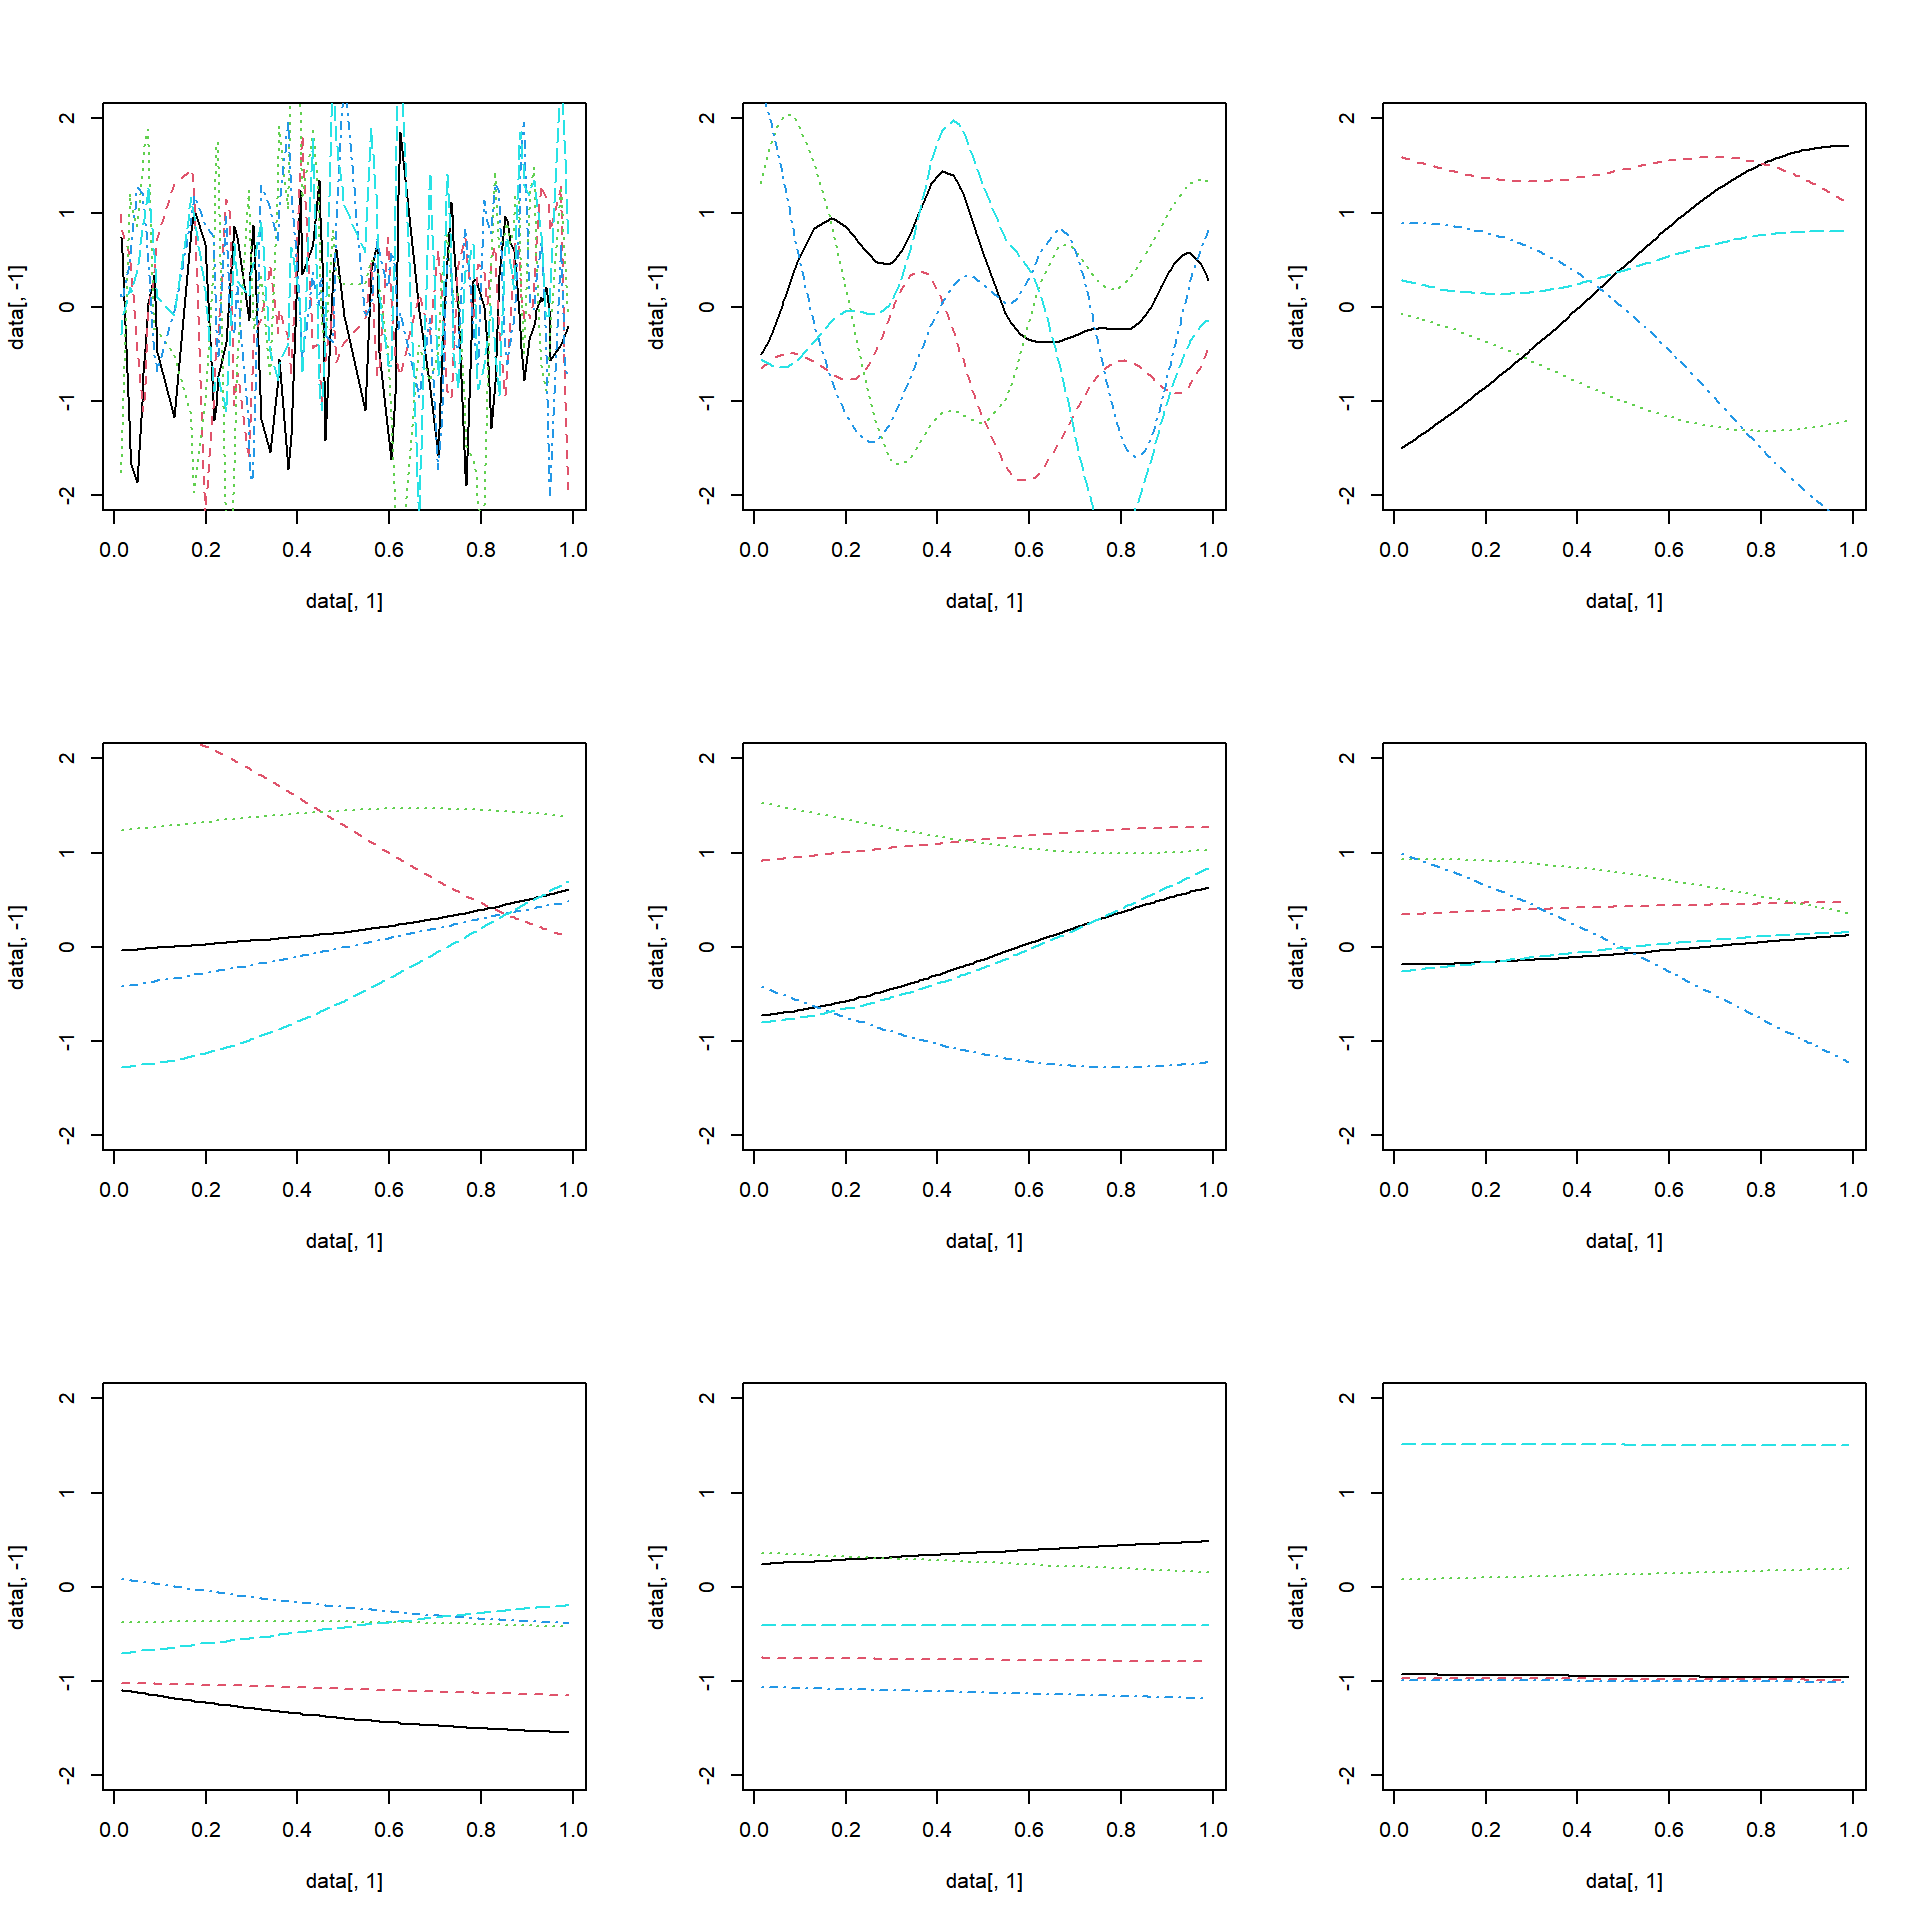
\includegraphics[width=1\linewidth]{04_gaussian_ch4_files/figure-latex/unnamed-chunk-3-1} \end{center}

\begin{Shaded}
\begin{Highlighting}[]
\FunctionTok{par}\NormalTok{(op)}
\end{Highlighting}
\end{Shaded}

\begin{Shaded}
\begin{Highlighting}[]
\NormalTok{get\_se\_Sigma }\OtherTok{\textless{}{-}} \ControlFlowTok{function}\NormalTok{(X1, X2, }\AttributeTok{l =} \DecValTok{1}\NormalTok{) \{}
\NormalTok{  Sigma }\OtherTok{\textless{}{-}} \FunctionTok{matrix}\NormalTok{(}\FunctionTok{rep}\NormalTok{(}\DecValTok{0}\NormalTok{, }\FunctionTok{length}\NormalTok{(X1) }\SpecialCharTok{*} \FunctionTok{length}\NormalTok{(X2)), }
                  \AttributeTok{nrow =} \FunctionTok{length}\NormalTok{(X1))}
  
  \ControlFlowTok{for}\NormalTok{ (i }\ControlFlowTok{in} \DecValTok{1}\SpecialCharTok{:}\FunctionTok{nrow}\NormalTok{(Sigma)) \{}
    \ControlFlowTok{for}\NormalTok{ (j }\ControlFlowTok{in} \DecValTok{1}\SpecialCharTok{:}\FunctionTok{ncol}\NormalTok{(Sigma)) \{}
\NormalTok{      Sigma[i, j] }\OtherTok{\textless{}{-}} \FunctionTok{exp}\NormalTok{(}\SpecialCharTok{{-}}\FloatTok{0.5} \SpecialCharTok{*}\NormalTok{ (}\FunctionTok{abs}\NormalTok{(X1[i] }\SpecialCharTok{{-}}\NormalTok{ X2[j]) }\SpecialCharTok{/}\NormalTok{ l)}\SpecialCharTok{\^{}}\DecValTok{2}\NormalTok{)}
\NormalTok{    \}}
\NormalTok{  \}}
  \FunctionTok{return}\NormalTok{(Sigma)}
\NormalTok{\}}
\end{Highlighting}
\end{Shaded}

\hypertarget{the-matern-class-of-covariance-functions}{%
\paragraph{The Matern Class of Covariance
Functions}\label{the-matern-class-of-covariance-functions}}

\[
k_{Matern}(r) = \frac {2^{1-\nu}} {\Gamma(\nu)} 
\Big( \frac {\sqrt{2\nu }r} l \Big)^ \nu
K_\nu \Big(\frac {\sqrt{2\nu }r} {l}\Big)
\ \ \ \ (4.14)
\]

\(K_{\nu}\) is a modified Bessel function!! Check what is a
\href{https://mathworld.wolfram.com/BesselFunctionoftheFirstKind.html}{Bessel
function}

\[
S(s) = \frac {2^D \pi^{D/2} \Gamma (\nu + D/2)(2\nu)^\nu}
{\Gamma(\nu)l^{2\nu}}
\Big(\frac {2\nu} {l^2} + 4\pi^2s^2\Big)^{-(\nu + D/2)} 
\ \ \ \ (4.15)
\]

\[
k_{\nu=p+1/2}(r) = 
exp \Big(- \frac {\sqrt{2\nu} r} l\Big) 
\frac {\Gamma(p+1)} {\Gamma(2p+ 1)}
\sum^p_{i=0}
\frac {(p + i)!} {i!(p - i)!}
\Big(\frac {\sqrt {8\nu}r } l\Big) ^ {p-i}
\ \ \ \ (4.16)
\]

\[
k_{\nu=1/2}(r) = exp(-\frac r l) \ \ \ \ (4.17a)\\ 
k_{\nu=3/2}(r) = \Big(1 + \frac {\sqrt 3r} l \Big)
exp \Big(- \frac {\sqrt 3r} {l}\Big) \ \ \ \ (4.17b)\\ 
k_{\nu=5/2}(r) = \Big(1 + \frac {\sqrt 5r} l + 
\frac {5r^2} {3l^2}\Big) exp \Big(- \frac {\sqrt 5r} l\Big)
\ \ \ \ (4.17c)
\]

\begin{Shaded}
\begin{Highlighting}[]
\DocumentationTok{\#\# change the scale length {-}{-}{-}{-}{-}{-}{-}{-}{-}{-}{-}{-}{-}{-}{-}{-}{-}{-}{-}{-}{-}{-}{-}{-}{-}{-}{-}{-}{-}{-}{-}{-}{-}{-}{-}{-}{-}{-}{-}{-}{-}{-}{-}{-}{-}}
\NormalTok{r }\OtherTok{=} \FunctionTok{seq}\NormalTok{(}\DecValTok{0}\NormalTok{, }\DecValTok{3}\NormalTok{, }\AttributeTok{len =} \DecValTok{100}\NormalTok{)}
\NormalTok{l1 }\OtherTok{\textless{}{-}} \FunctionTok{c}\NormalTok{(}\FloatTok{0.01}\NormalTok{, }\FloatTok{0.1}\NormalTok{,  }\FloatTok{0.5}\NormalTok{,}
         \FloatTok{0.9}\NormalTok{,   }\DecValTok{1}\NormalTok{,  }\FloatTok{1.2}\NormalTok{, }
           \DecValTok{2}\NormalTok{,   }\DecValTok{5}\NormalTok{,  }\DecValTok{10}\NormalTok{)}
\NormalTok{kernel\_mat }\OtherTok{\textless{}{-}} \FunctionTok{matrix}\NormalTok{(}\AttributeTok{data =} \ConstantTok{NA}\NormalTok{, }\AttributeTok{nrow =} \FunctionTok{length}\NormalTok{(l1), }\AttributeTok{ncol =} \FunctionTok{length}\NormalTok{(r))}
\ControlFlowTok{for}\NormalTok{ (i }\ControlFlowTok{in} \DecValTok{1}\SpecialCharTok{:}\DecValTok{9}\NormalTok{) \{}
  \ControlFlowTok{for}\NormalTok{ (j }\ControlFlowTok{in} \DecValTok{1}\SpecialCharTok{:}\FunctionTok{length}\NormalTok{(r)) \{}
\NormalTok{    kernel\_mat[i, j] }\OtherTok{\textless{}{-}}\NormalTok{ geoR}\SpecialCharTok{::}\FunctionTok{matern}\NormalTok{(r[j], }\AttributeTok{phi =}\NormalTok{ l1[i], }\AttributeTok{kappa =} \DecValTok{1}\NormalTok{)}
\NormalTok{  \}}
\NormalTok{\}}
\FunctionTok{matplot}\NormalTok{(r, }\FunctionTok{t}\NormalTok{(kernel\_mat), }\StringTok{"l"}\NormalTok{, }
        \AttributeTok{xlab =} \StringTok{"input, x"}\NormalTok{, }\AttributeTok{ylab =} \StringTok{"output, y"}\NormalTok{)}
\end{Highlighting}
\end{Shaded}

\begin{center}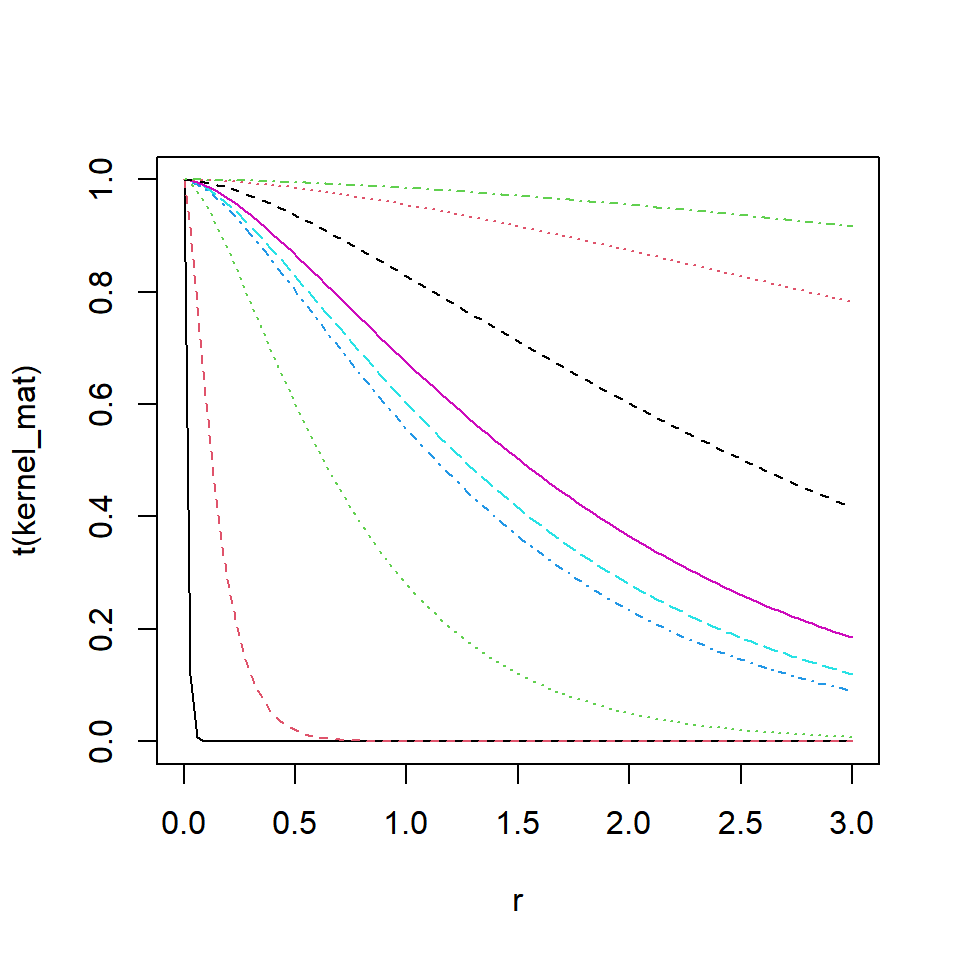
\includegraphics[width=0.4\linewidth]{04_gaussian_ch4_files/figure-latex/matern matrix kernel-1} \end{center}

\begin{Shaded}
\begin{Highlighting}[]
\DocumentationTok{\#\# change the degree of freedom {-}{-}{-}{-}{-}{-}{-}{-}{-}{-}{-}{-}{-}{-}{-}{-}{-}{-}{-}{-}{-}{-}{-}{-}{-}{-}{-}{-}{-}{-}{-}{-}{-}{-}{-}{-}{-}{-}{-}{-}{-}{-}{-}{-}{-}}

\NormalTok{nu }\OtherTok{\textless{}{-}} \FunctionTok{c}\NormalTok{(}\FloatTok{0.001}\NormalTok{, }\FloatTok{0.1}\NormalTok{, }\FloatTok{0.5}\NormalTok{,}
        \DecValTok{1}\NormalTok{, }\DecValTok{2}\NormalTok{, }\DecValTok{5}\NormalTok{, }
        \DecValTok{10}\NormalTok{, }\DecValTok{100}\NormalTok{, }\DecValTok{1000}\NormalTok{)}
\NormalTok{kernel\_mat\_df }\OtherTok{\textless{}{-}} \FunctionTok{matrix}\NormalTok{(}\AttributeTok{data =} \ConstantTok{NA}\NormalTok{, }\AttributeTok{nrow =} \FunctionTok{length}\NormalTok{(l1), }\AttributeTok{ncol =} \FunctionTok{length}\NormalTok{(r))}
\ControlFlowTok{for}\NormalTok{ (i }\ControlFlowTok{in} \DecValTok{1}\SpecialCharTok{:}\DecValTok{9}\NormalTok{) \{}
  \ControlFlowTok{for}\NormalTok{ (j }\ControlFlowTok{in} \DecValTok{1}\SpecialCharTok{:}\FunctionTok{length}\NormalTok{(r)) \{}
\NormalTok{    kernel\_mat\_df[i, j] }\OtherTok{\textless{}{-}}\NormalTok{ geoR}\SpecialCharTok{::}\FunctionTok{matern}\NormalTok{(r[j], }
                                        \AttributeTok{phi =} \DecValTok{1}\SpecialCharTok{/}\NormalTok{(}\FunctionTok{sqrt}\NormalTok{(}\DecValTok{2} \SpecialCharTok{*}\NormalTok{ nu[i])), }
                                        \AttributeTok{kappa =}\NormalTok{ nu[i])}
\NormalTok{  \}}
\NormalTok{\}}
\FunctionTok{matplot}\NormalTok{(r, }\FunctionTok{t}\NormalTok{(kernel\_mat\_df), }
        \AttributeTok{xlab =} \StringTok{"input, x"}\NormalTok{, }\AttributeTok{ylab =} \StringTok{"output, y"}\NormalTok{, }
        \StringTok{"l"}\NormalTok{)}
\FunctionTok{abline}\NormalTok{(}\AttributeTok{v =} \FloatTok{1.95}\NormalTok{, }\AttributeTok{lty =} \StringTok{"dashed"}\NormalTok{, }\AttributeTok{col =} \StringTok{"grey"}\NormalTok{)}
\end{Highlighting}
\end{Shaded}

\begin{center}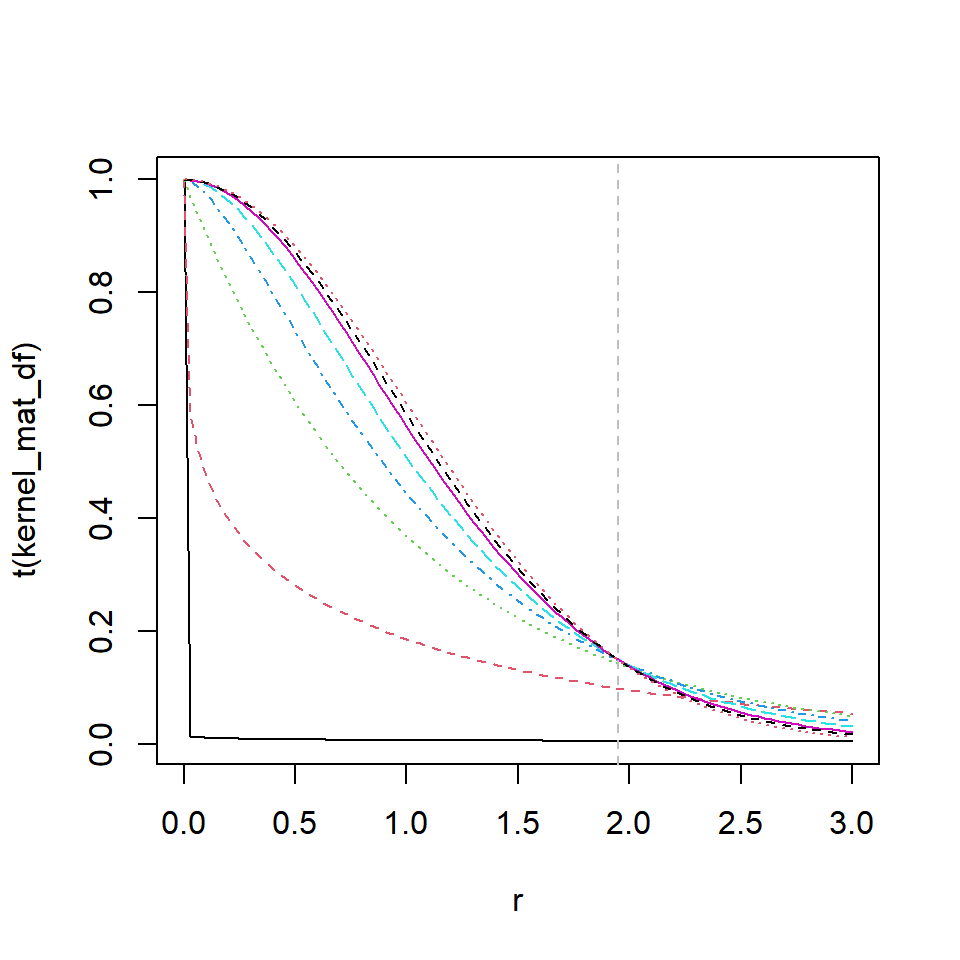
\includegraphics[width=0.4\linewidth]{04_gaussian_ch4_files/figure-latex/matern matrix kernel-2} \end{center}

\begin{Shaded}
\begin{Highlighting}[]
\NormalTok{l1 }\OtherTok{\textless{}{-}} \FunctionTok{c}\NormalTok{(}\FloatTok{0.01}\NormalTok{, }\FloatTok{0.1}\NormalTok{,  }\FloatTok{0.5}\NormalTok{,}
         \FloatTok{0.9}\NormalTok{,   }\DecValTok{1}\NormalTok{,  }\FloatTok{1.2}\NormalTok{, }
           \DecValTok{2}\NormalTok{,   }\DecValTok{5}\NormalTok{,  }\DecValTok{10}\NormalTok{)}
\NormalTok{op }\OtherTok{\textless{}{-}} \FunctionTok{par}\NormalTok{(}\AttributeTok{mfrow =} \FunctionTok{c}\NormalTok{(}\DecValTok{3}\NormalTok{, }\DecValTok{3}\NormalTok{))}
\NormalTok{x }\OtherTok{\textless{}{-}} \FunctionTok{runif}\NormalTok{(}\DecValTok{100}\NormalTok{)}
\NormalTok{d }\OtherTok{\textless{}{-}} \FunctionTok{abs}\NormalTok{(}\FunctionTok{outer}\NormalTok{(x, x, }\AttributeTok{FUN =} \StringTok{"{-}"}\NormalTok{))}
\ControlFlowTok{for}\NormalTok{ (i }\ControlFlowTok{in} \DecValTok{1}\SpecialCharTok{:}\DecValTok{9}\NormalTok{) \{}
  \DocumentationTok{\#\# \textbackslash{}phi is the l scale in GP book}
  \DocumentationTok{\#\# \textbackslash{}kappa is the \textbackslash{}mu in GP book}
\NormalTok{  kernel\_mat }\OtherTok{\textless{}{-}}\NormalTok{ geoR}\SpecialCharTok{::}\FunctionTok{matern}\NormalTok{(d, }\AttributeTok{phi =}\NormalTok{ l1[i], }\AttributeTok{kappa =} \DecValTok{1}\NormalTok{) }
\NormalTok{  sim }\OtherTok{\textless{}{-}}\NormalTok{ mvtnorm}\SpecialCharTok{::}\FunctionTok{rmvnorm}\NormalTok{(}\DecValTok{10}\NormalTok{, }\AttributeTok{sigma =}\NormalTok{ kernel\_mat)}
\NormalTok{  data }\OtherTok{\textless{}{-}} \FunctionTok{cbind}\NormalTok{(x, }\FunctionTok{t}\NormalTok{(sim)) }\SpecialCharTok{\%\textgreater{}\%} 
    \FunctionTok{data.frame}\NormalTok{() }\SpecialCharTok{\%\textgreater{}\%}
    \FunctionTok{arrange}\NormalTok{(}\AttributeTok{by =}\NormalTok{ x)}
  \FunctionTok{matplot}\NormalTok{(data[, }\DecValTok{1}\NormalTok{], data[, }\SpecialCharTok{{-}}\DecValTok{1}\NormalTok{], }
          \AttributeTok{xlab =} \StringTok{"input, x"}\NormalTok{, }\AttributeTok{ylab =} \StringTok{"output, y"}\NormalTok{,}
          \StringTok{"l"}\NormalTok{, }\AttributeTok{ylim =} \FunctionTok{c}\NormalTok{(}\SpecialCharTok{{-}}\DecValTok{2}\NormalTok{, }\DecValTok{2}\NormalTok{))}
\NormalTok{\}}
\end{Highlighting}
\end{Shaded}

\begin{center}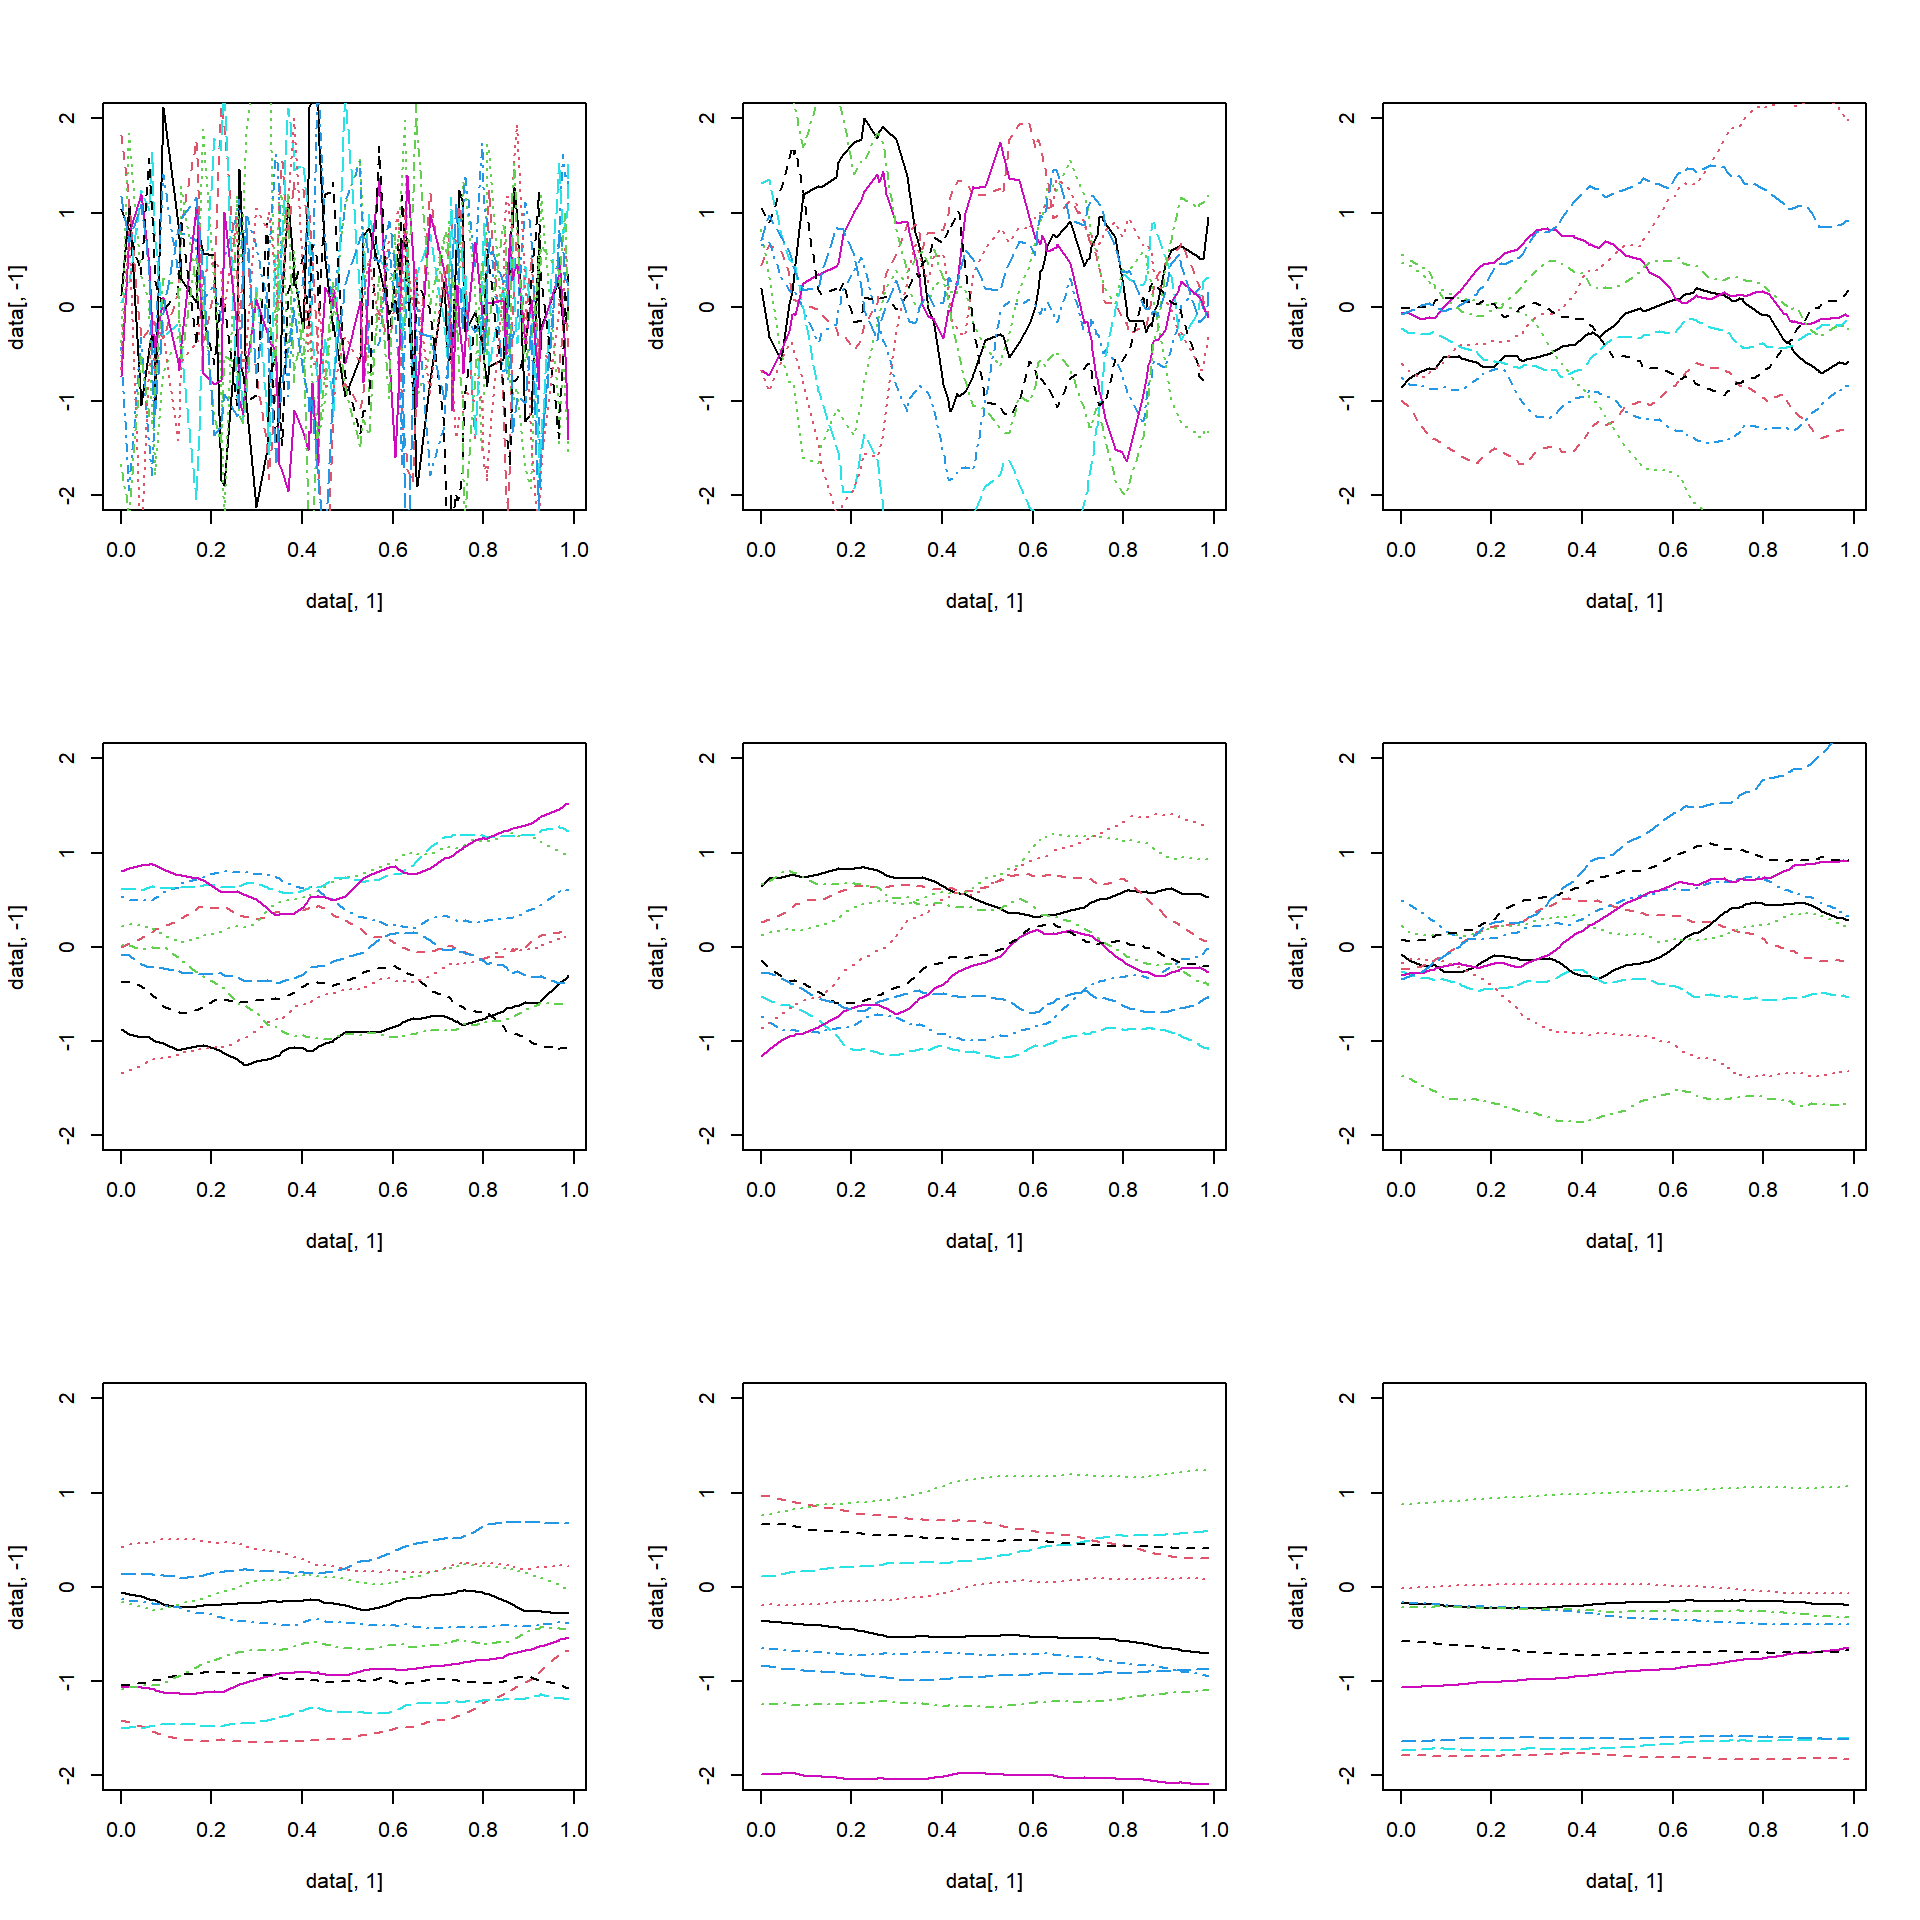
\includegraphics[width=1\linewidth]{04_gaussian_ch4_files/figure-latex/matern scale-1} \end{center}

\begin{Shaded}
\begin{Highlighting}[]
\FunctionTok{par}\NormalTok{(op)}
\end{Highlighting}
\end{Shaded}

\begin{Shaded}
\begin{Highlighting}[]
\FunctionTok{set.seed}\NormalTok{(}\DecValTok{555}\NormalTok{)}
\NormalTok{nu }\OtherTok{\textless{}{-}} \FunctionTok{c}\NormalTok{(}\FloatTok{0.1}\NormalTok{, }\FloatTok{0.5}\NormalTok{, }\FloatTok{0.9}\NormalTok{, }\DecValTok{1}\NormalTok{, }
        \FloatTok{1.5}\NormalTok{, }\DecValTok{2}\NormalTok{, }\DecValTok{5}\NormalTok{, }\DecValTok{10}\NormalTok{, }\DecValTok{20}\NormalTok{)}
\NormalTok{op }\OtherTok{\textless{}{-}} \FunctionTok{par}\NormalTok{(}\AttributeTok{mfrow =} \FunctionTok{c}\NormalTok{(}\DecValTok{3}\NormalTok{, }\DecValTok{3}\NormalTok{))}
\NormalTok{x }\OtherTok{\textless{}{-}} \FunctionTok{runif}\NormalTok{(}\DecValTok{100}\NormalTok{)}
\NormalTok{d }\OtherTok{\textless{}{-}} \FunctionTok{abs}\NormalTok{(}\FunctionTok{outer}\NormalTok{(x, x, }\AttributeTok{FUN =} \StringTok{"{-}"}\NormalTok{))}
\ControlFlowTok{for}\NormalTok{ (i }\ControlFlowTok{in} \DecValTok{1}\SpecialCharTok{:}\DecValTok{9}\NormalTok{) \{}
  \DocumentationTok{\#\# \textbackslash{}phi is the l / (sqrt(2*\textbackslash{}kappa))  scale in GP book}
  \DocumentationTok{\#\# \textbackslash{}kappa is the \textbackslash{}nu in GP book}
\NormalTok{  kernel\_mat }\OtherTok{\textless{}{-}}\NormalTok{ geoR}\SpecialCharTok{::}\FunctionTok{matern}\NormalTok{(d, }\AttributeTok{phi =} \DecValTok{1}\SpecialCharTok{/}\NormalTok{(}\FunctionTok{sqrt}\NormalTok{(}\DecValTok{2} \SpecialCharTok{*}\NormalTok{ nu[i])), }\AttributeTok{kappa =}\NormalTok{ nu[i]) }
\NormalTok{  kernel\_mat }\OtherTok{\textless{}{-}} \FunctionTok{get\_symm}\NormalTok{(}\FunctionTok{t}\NormalTok{(kernel\_mat))}
\NormalTok{  kernel\_mat[}\FunctionTok{is.na}\NormalTok{(kernel\_mat)] }\OtherTok{\textless{}{-}} \DecValTok{0} 
  
\NormalTok{  sim }\OtherTok{\textless{}{-}}\NormalTok{ mvtnorm}\SpecialCharTok{::}\FunctionTok{rmvnorm}\NormalTok{(}\DecValTok{5}\NormalTok{, }\AttributeTok{sigma =}\NormalTok{ kernel\_mat)}
\NormalTok{  data }\OtherTok{\textless{}{-}} \FunctionTok{cbind}\NormalTok{(x, }\FunctionTok{t}\NormalTok{(sim)) }\SpecialCharTok{\%\textgreater{}\%} 
    \FunctionTok{data.frame}\NormalTok{() }\SpecialCharTok{\%\textgreater{}\%}
    \FunctionTok{arrange}\NormalTok{(}\AttributeTok{by =}\NormalTok{ x)}
  \FunctionTok{matplot}\NormalTok{(data[, }\DecValTok{1}\NormalTok{], data[, }\SpecialCharTok{{-}}\DecValTok{1}\NormalTok{], }
          \AttributeTok{xlab =} \StringTok{"input, x"}\NormalTok{, }\AttributeTok{ylab =} \StringTok{"output, y"}\NormalTok{,}
          \StringTok{"l"}\NormalTok{, }\AttributeTok{ylim =} \FunctionTok{c}\NormalTok{(}\SpecialCharTok{{-}}\DecValTok{2}\NormalTok{, }\DecValTok{2}\NormalTok{))}
\NormalTok{\}}
\end{Highlighting}
\end{Shaded}

\begin{center}\includegraphics[width=1\linewidth]{04_gaussian_ch4_files/figure-latex/matern df-1} \end{center}

\begin{Shaded}
\begin{Highlighting}[]
\FunctionTok{par}\NormalTok{(op)}

\DocumentationTok{\#\# use besselK() for the Bessel functions}
\end{Highlighting}
\end{Shaded}

Ornstein-Uhlenbeck Process and Exponential Covariance Function

\begin{Shaded}
\begin{Highlighting}[]
\NormalTok{l1 }\OtherTok{\textless{}{-}} \FunctionTok{c}\NormalTok{(}\FloatTok{0.01}\NormalTok{, }\FloatTok{0.1}\NormalTok{,  }\FloatTok{0.5}\NormalTok{,}
         \FloatTok{0.9}\NormalTok{,   }\DecValTok{1}\NormalTok{,  }\FloatTok{1.2}\NormalTok{, }
           \DecValTok{2}\NormalTok{,   }\DecValTok{5}\NormalTok{,  }\DecValTok{10}\NormalTok{)}

\NormalTok{op }\OtherTok{\textless{}{-}} \FunctionTok{par}\NormalTok{(}\AttributeTok{mfrow =} \FunctionTok{c}\NormalTok{(}\DecValTok{3}\NormalTok{, }\DecValTok{3}\NormalTok{))}
\NormalTok{x }\OtherTok{\textless{}{-}} \FunctionTok{runif}\NormalTok{(}\DecValTok{100}\NormalTok{)}
\NormalTok{d }\OtherTok{\textless{}{-}} \FunctionTok{abs}\NormalTok{(}\FunctionTok{outer}\NormalTok{(x, x, }\AttributeTok{FUN =} \StringTok{"{-}"}\NormalTok{))}

\ControlFlowTok{for}\NormalTok{ (i }\ControlFlowTok{in} \DecValTok{1}\SpecialCharTok{:}\DecValTok{9}\NormalTok{) \{}
\NormalTok{  kernel\_ou }\OtherTok{\textless{}{-}} \FunctionTok{exp}\NormalTok{(}\SpecialCharTok{{-}}\NormalTok{d }\SpecialCharTok{/}\NormalTok{ l1[i]) }
\NormalTok{  sim }\OtherTok{\textless{}{-}}\NormalTok{ mvtnorm}\SpecialCharTok{::}\FunctionTok{rmvnorm}\NormalTok{(}\DecValTok{5}\NormalTok{, }\AttributeTok{sigma =}\NormalTok{ kernel\_ou)}
\NormalTok{  data }\OtherTok{\textless{}{-}} \FunctionTok{cbind}\NormalTok{(x, }\FunctionTok{t}\NormalTok{(sim)) }\SpecialCharTok{\%\textgreater{}\%} 
    \FunctionTok{data.frame}\NormalTok{() }\SpecialCharTok{\%\textgreater{}\%}
    \FunctionTok{arrange}\NormalTok{(}\AttributeTok{by =}\NormalTok{ x)}
  \FunctionTok{matplot}\NormalTok{(data[, }\DecValTok{1}\NormalTok{], data[, }\SpecialCharTok{{-}}\DecValTok{1}\NormalTok{], }
          \AttributeTok{xlab =} \StringTok{"input, x"}\NormalTok{, }\AttributeTok{ylab =} \StringTok{"output, y"}\NormalTok{, }
          \StringTok{"l"}\NormalTok{, }\AttributeTok{ylim =} \FunctionTok{c}\NormalTok{(}\SpecialCharTok{{-}}\DecValTok{2}\NormalTok{, }\DecValTok{2}\NormalTok{))}
\NormalTok{\}}
\end{Highlighting}
\end{Shaded}

\begin{center}\includegraphics[width=1\linewidth]{04_gaussian_ch4_files/figure-latex/ornstein-uhlenbeck-1} \end{center}

\begin{Shaded}
\begin{Highlighting}[]
\FunctionTok{par}\NormalTok{(op)}
\end{Highlighting}
\end{Shaded}

\hypertarget{the-gamma-exponential-covariance-function}{%
\paragraph{\texorpdfstring{The \(\gamma\)-exponential Covariance
Function}{The \textbackslash gamma-exponential Covariance Function}}\label{the-gamma-exponential-covariance-function}}

\[
k(r) = exp\Big( - \big(\frac r l\big) \Big)^\gamma,\  for\  0 < \gamma \neq 2
\ \ \ \ (4.18)
\]

\begin{Shaded}
\begin{Highlighting}[]
\DocumentationTok{\#\# change the scale length {-}{-}{-}{-}{-}{-}{-}{-}{-}{-}{-}{-}{-}{-}{-}{-}{-}{-}{-}{-}{-}{-}{-}{-}{-}{-}{-}{-}{-}{-}{-}{-}{-}{-}{-}{-}{-}{-}{-}{-}{-}{-}{-}{-}{-}}
\NormalTok{l1 }\OtherTok{\textless{}{-}} \FunctionTok{c}\NormalTok{(}\FloatTok{0.01}\NormalTok{, }\FloatTok{0.1}\NormalTok{,  }\FloatTok{0.5}\NormalTok{,}
         \FloatTok{0.9}\NormalTok{,   }\DecValTok{1}\NormalTok{,  }\FloatTok{1.2}\NormalTok{, }
           \DecValTok{2}\NormalTok{,   }\DecValTok{5}\NormalTok{,  }\DecValTok{10}\NormalTok{)}
\NormalTok{kernel\_gamma }\OtherTok{\textless{}{-}} \FunctionTok{matrix}\NormalTok{(}\AttributeTok{data =} \ConstantTok{NA}\NormalTok{, }\AttributeTok{nrow =} \FunctionTok{length}\NormalTok{(l1), }\AttributeTok{ncol =} \FunctionTok{length}\NormalTok{(r))}
\ControlFlowTok{for}\NormalTok{ (i }\ControlFlowTok{in} \DecValTok{1}\SpecialCharTok{:}\DecValTok{9}\NormalTok{) \{}
  \ControlFlowTok{for}\NormalTok{ (j }\ControlFlowTok{in} \DecValTok{1}\SpecialCharTok{:}\FunctionTok{length}\NormalTok{(r)) \{}
\NormalTok{    kernel\_gamma[i, j] }\OtherTok{\textless{}{-}} \FunctionTok{exp}\NormalTok{(}\SpecialCharTok{{-}}\NormalTok{ (r[j] }\SpecialCharTok{/}\NormalTok{ l1[i])}\SpecialCharTok{\^{}}\FloatTok{0.5}\NormalTok{) }
\NormalTok{  \}}
\NormalTok{\}}
\FunctionTok{matplot}\NormalTok{(r, }\FunctionTok{t}\NormalTok{(kernel\_gamma), }
        \AttributeTok{xlab =} \StringTok{"input, x"}\NormalTok{, }\AttributeTok{ylab =} \StringTok{"output, y"}\NormalTok{, }\StringTok{"l"}\NormalTok{)}
\end{Highlighting}
\end{Shaded}

\begin{center}\includegraphics[width=0.4\linewidth]{04_gaussian_ch4_files/figure-latex/unnamed-chunk-5-1} \end{center}

\begin{Shaded}
\begin{Highlighting}[]
\DocumentationTok{\#\# change the degree of freedom {-}{-}{-}{-}{-}{-}{-}{-}{-}{-}{-}{-}{-}{-}{-}{-}{-}{-}{-}{-}{-}{-}{-}{-}{-}{-}{-}{-}{-}{-}{-}{-}{-}{-}{-}{-}{-}{-}{-}{-}{-}{-}{-}{-}{-}}
\NormalTok{r }\OtherTok{=} \FunctionTok{seq}\NormalTok{(}\DecValTok{0}\NormalTok{, }\DecValTok{3}\NormalTok{, }\AttributeTok{len =} \DecValTok{1000}\NormalTok{)}
\NormalTok{gamma }\OtherTok{\textless{}{-}} \FunctionTok{c}\NormalTok{(}\FloatTok{0.001}\NormalTok{, }\FloatTok{0.1}\NormalTok{, }\FloatTok{0.5}\NormalTok{,}
          \DecValTok{1}\NormalTok{, }\FloatTok{1.5}\NormalTok{, }\DecValTok{2}\NormalTok{)}
\NormalTok{kernel\_gammaex }\OtherTok{\textless{}{-}} \FunctionTok{matrix}\NormalTok{(}\AttributeTok{data =} \ConstantTok{NA}\NormalTok{, }\AttributeTok{nrow =} \DecValTok{6}\NormalTok{, }\AttributeTok{ncol =} \FunctionTok{length}\NormalTok{(r))}
\ControlFlowTok{for}\NormalTok{ (i }\ControlFlowTok{in} \DecValTok{1}\SpecialCharTok{:}\DecValTok{6}\NormalTok{) \{}
  \ControlFlowTok{for}\NormalTok{ (j }\ControlFlowTok{in} \DecValTok{1}\SpecialCharTok{:}\FunctionTok{length}\NormalTok{(r)) \{}
\NormalTok{    kernel\_gammaex[i, j] }\OtherTok{\textless{}{-}} \FunctionTok{exp}\NormalTok{(}\SpecialCharTok{{-}}\NormalTok{(r[j])}\SpecialCharTok{\^{}}\NormalTok{gamma[i])}
\NormalTok{  \}}
\NormalTok{\}}
\FunctionTok{matplot}\NormalTok{(r, }\FunctionTok{t}\NormalTok{(kernel\_gammaex), }
        \AttributeTok{xlab =} \StringTok{"input, x"}\NormalTok{, }\AttributeTok{ylab =} \StringTok{"output, y"}\NormalTok{,}
        \StringTok{"l"}\NormalTok{)}
\FunctionTok{abline}\NormalTok{(}\AttributeTok{v =} \DecValTok{1}\NormalTok{, }\AttributeTok{h =} \FloatTok{0.365}\NormalTok{, }\AttributeTok{lty =} \StringTok{"dashed"}\NormalTok{, }\AttributeTok{col =} \StringTok{"grey"}\NormalTok{)}
\end{Highlighting}
\end{Shaded}

\begin{center}\includegraphics[width=0.4\linewidth]{04_gaussian_ch4_files/figure-latex/unnamed-chunk-6-1} \end{center}

\begin{Shaded}
\begin{Highlighting}[]
\NormalTok{l1 }\OtherTok{\textless{}{-}} \FunctionTok{c}\NormalTok{(}\FloatTok{0.01}\NormalTok{, }\FloatTok{0.1}\NormalTok{,  }\FloatTok{0.5}\NormalTok{,}
         \FloatTok{0.9}\NormalTok{,   }\DecValTok{1}\NormalTok{,  }\FloatTok{1.2}\NormalTok{, }
           \DecValTok{2}\NormalTok{,   }\DecValTok{5}\NormalTok{,  }\DecValTok{10}\NormalTok{)}

\NormalTok{op }\OtherTok{\textless{}{-}} \FunctionTok{par}\NormalTok{(}\AttributeTok{mfrow =} \FunctionTok{c}\NormalTok{(}\DecValTok{3}\NormalTok{, }\DecValTok{3}\NormalTok{))}
\NormalTok{x }\OtherTok{\textless{}{-}} \FunctionTok{runif}\NormalTok{(}\DecValTok{100}\NormalTok{)}
\NormalTok{d }\OtherTok{\textless{}{-}} \FunctionTok{abs}\NormalTok{(}\FunctionTok{outer}\NormalTok{(x, x, }\AttributeTok{FUN =} \StringTok{"{-}"}\NormalTok{))}

\ControlFlowTok{for}\NormalTok{ (i }\ControlFlowTok{in} \DecValTok{1}\SpecialCharTok{:}\DecValTok{9}\NormalTok{) \{}
\NormalTok{  kernel\_gammaex }\OtherTok{\textless{}{-}} \FunctionTok{exp}\NormalTok{(}\SpecialCharTok{{-}}\NormalTok{ (d }\SpecialCharTok{/}\NormalTok{ l1[i])}\SpecialCharTok{\^{}}\FloatTok{0.5}\NormalTok{) }
\NormalTok{  sim }\OtherTok{\textless{}{-}}\NormalTok{ mvtnorm}\SpecialCharTok{::}\FunctionTok{rmvnorm}\NormalTok{(}\DecValTok{5}\NormalTok{, }\AttributeTok{sigma =}\NormalTok{ kernel\_gammaex)}
\NormalTok{  data }\OtherTok{\textless{}{-}} \FunctionTok{cbind}\NormalTok{(x, }\FunctionTok{t}\NormalTok{(sim)) }\SpecialCharTok{\%\textgreater{}\%} 
    \FunctionTok{data.frame}\NormalTok{() }\SpecialCharTok{\%\textgreater{}\%}
    \FunctionTok{arrange}\NormalTok{(}\AttributeTok{by =}\NormalTok{ x)}
  \FunctionTok{matplot}\NormalTok{(data[, }\DecValTok{1}\NormalTok{], data[, }\SpecialCharTok{{-}}\DecValTok{1}\NormalTok{], }
          \AttributeTok{xlab =} \StringTok{"input, x"}\NormalTok{, }\AttributeTok{ylab =} \StringTok{"output, y"}\NormalTok{,}
          \StringTok{"l"}\NormalTok{, }\AttributeTok{ylim =} \FunctionTok{c}\NormalTok{(}\SpecialCharTok{{-}}\DecValTok{2}\NormalTok{, }\DecValTok{2}\NormalTok{))}
\NormalTok{\}}
\end{Highlighting}
\end{Shaded}

\begin{center}\includegraphics[width=1\linewidth]{04_gaussian_ch4_files/figure-latex/gamma exponential-1} \end{center}

\begin{Shaded}
\begin{Highlighting}[]
\FunctionTok{par}\NormalTok{(op)}
\end{Highlighting}
\end{Shaded}

\hypertarget{rational-quadratic-covariance-function}{%
\paragraph{Rational Quadratic Covariance
Function}\label{rational-quadratic-covariance-function}}

\[
k_{RQ}(r) = \Big(1 + \frac {r^2} {2\alpha l^2} \Big)^{-\alpha}
\ \ \ \ (4.19)
\]

\[
k_{RQ}(r) = \int p(\tau|\alpha,\ \beta)k_{SE}(r|\tau) d\tau\\
\propto \int \tau^{\alpha -1} 
exp \Big(- \frac {\alpha \tau} \beta \Big)
exp \Big(- \frac {\tau r^2} 2\Big) d\tau\\
\propto \Big(1 + \frac {r^2} {2\alpha l^2}\Big)^{-\alpha}
\ \ \ \ (4.20)
\]

\begin{Shaded}
\begin{Highlighting}[]
\DocumentationTok{\#\# change the alpha {-}{-}{-}{-}{-}{-}{-}{-}{-}{-}{-}{-}{-}{-}{-}{-}{-}{-}{-}{-}{-}{-}{-}{-}{-}{-}{-}{-}{-}{-}{-}{-}{-}{-}{-}{-}{-}{-}{-}{-}{-}{-}{-}{-}{-}}
\NormalTok{alpha }\OtherTok{\textless{}{-}} \FunctionTok{c}\NormalTok{(}\FloatTok{0.001}\NormalTok{, }\FloatTok{0.1}\NormalTok{, }\FloatTok{0.5}\NormalTok{,}
          \DecValTok{1}\NormalTok{, }\DecValTok{2}\NormalTok{, }\DecValTok{5}\NormalTok{,}
          \DecValTok{10}\NormalTok{, }\DecValTok{100}\NormalTok{, }\DecValTok{1000}\NormalTok{)}
\NormalTok{kernel\_rq }\OtherTok{\textless{}{-}} \FunctionTok{matrix}\NormalTok{(}\AttributeTok{data =} \ConstantTok{NA}\NormalTok{, }\AttributeTok{nrow =} \FunctionTok{length}\NormalTok{(alpha), }\AttributeTok{ncol =} \FunctionTok{length}\NormalTok{(r))}
\ControlFlowTok{for}\NormalTok{ (i }\ControlFlowTok{in} \DecValTok{1}\SpecialCharTok{:}\DecValTok{9}\NormalTok{) \{}
  \ControlFlowTok{for}\NormalTok{ (j }\ControlFlowTok{in} \DecValTok{1}\SpecialCharTok{:}\FunctionTok{length}\NormalTok{(r)) \{}
\NormalTok{    kernel\_rq[i, j] }\OtherTok{\textless{}{-}}\NormalTok{ (}\DecValTok{1} \SpecialCharTok{+}\NormalTok{ r[j]}\SpecialCharTok{\^{}}\DecValTok{2} \SpecialCharTok{/}\NormalTok{ (}\DecValTok{2} \SpecialCharTok{*}\NormalTok{ alpha[i]))}\SpecialCharTok{\^{}}\NormalTok{(}\SpecialCharTok{{-}}\NormalTok{alpha[i])}
\NormalTok{  \}}
\NormalTok{\}}
\FunctionTok{matplot}\NormalTok{(r, }\FunctionTok{t}\NormalTok{(kernel\_rq), }
        \AttributeTok{xlab =} \StringTok{"input, x"}\NormalTok{, }\AttributeTok{ylab =} \StringTok{"output, y"}\NormalTok{,}
        \StringTok{"l"}\NormalTok{)}
\end{Highlighting}
\end{Shaded}

\begin{center}\includegraphics[width=0.4\linewidth]{04_gaussian_ch4_files/figure-latex/unnamed-chunk-7-1} \end{center}

\begin{Shaded}
\begin{Highlighting}[]
\NormalTok{alpha }\OtherTok{\textless{}{-}} \FunctionTok{c}\NormalTok{(}\FloatTok{0.5}\NormalTok{, }\DecValTok{1}\NormalTok{, }\DecValTok{2}\NormalTok{, }
          \DecValTok{10}\NormalTok{, }\DecValTok{100}\NormalTok{, }\DecValTok{1000}\NormalTok{)}
\NormalTok{op }\OtherTok{\textless{}{-}} \FunctionTok{par}\NormalTok{(}\AttributeTok{mfrow =} \FunctionTok{c}\NormalTok{(}\DecValTok{3}\NormalTok{, }\DecValTok{3}\NormalTok{))}
\NormalTok{x }\OtherTok{\textless{}{-}} \FunctionTok{runif}\NormalTok{(}\DecValTok{1000}\NormalTok{)}
\NormalTok{d }\OtherTok{\textless{}{-}} \FunctionTok{abs}\NormalTok{(}\FunctionTok{outer}\NormalTok{(x, x, }\AttributeTok{FUN =} \StringTok{"{-}"}\NormalTok{))}

\ControlFlowTok{for}\NormalTok{ (i }\ControlFlowTok{in} \DecValTok{1}\SpecialCharTok{:}\DecValTok{6}\NormalTok{) \{}
\NormalTok{  kernel\_rq\_alpha }\OtherTok{\textless{}{-}}\NormalTok{ (}\DecValTok{1} \SpecialCharTok{+}\NormalTok{ d}\SpecialCharTok{\^{}}\DecValTok{2} \SpecialCharTok{/}\NormalTok{ (}\DecValTok{2} \SpecialCharTok{*}\NormalTok{ alpha[i]))}\SpecialCharTok{\^{}}\NormalTok{(}\SpecialCharTok{{-}}\NormalTok{alpha[i])}
\NormalTok{  sim }\OtherTok{\textless{}{-}}\NormalTok{ mvtnorm}\SpecialCharTok{::}\FunctionTok{rmvnorm}\NormalTok{(}\DecValTok{5}\NormalTok{, }\AttributeTok{sigma =}\NormalTok{ kernel\_rq\_alpha)}
\NormalTok{  data }\OtherTok{\textless{}{-}} \FunctionTok{cbind}\NormalTok{(x, }\FunctionTok{t}\NormalTok{(sim)) }\SpecialCharTok{\%\textgreater{}\%} 
    \FunctionTok{data.frame}\NormalTok{() }\SpecialCharTok{\%\textgreater{}\%}
    \FunctionTok{arrange}\NormalTok{(}\AttributeTok{by =}\NormalTok{ x)}
  \FunctionTok{matplot}\NormalTok{(data[, }\DecValTok{1}\NormalTok{], data[, }\SpecialCharTok{{-}}\DecValTok{1}\NormalTok{], }\StringTok{"l"}\NormalTok{)}
\NormalTok{\}}

\FunctionTok{par}\NormalTok{(op)}
\end{Highlighting}
\end{Shaded}

\begin{center}\includegraphics[width=1\linewidth]{04_gaussian_ch4_files/figure-latex/gamma rq-1} \end{center}

Piecewise Polynomial Covariance Functions with Compact Support

\[
k_{ppD,0}(r) = (1 - r)^j_+,\ \ 
where\ j = \lfloor \frac D 2 \rfloor 
+ q + 1 \ \ \ \ (4.21a)\\
k_{ppD,1}(r) = (1 - r)^{j+1}_{+}
\big((j + 1)r + 1\big)
\ \ \ \ (4.21b)\\
k_{ppD,2}(r) = (1 - r)^{j+2}_{+}
\big((j^2 + 4j + 3)r^2 + (3j + 6)r + 3\big)/3 \ \ \ \ (4.21c)\\
k_{ppD,3}(r) = (1 - r)^{j+3}_{+}
\big((j^3 + 9j^2 + 23j + 15)r^3+
(6j^2 + 36j + 45)r^2 + (15j + 45)r + 15\big)/15
\ \ \ \ (4.21d)
\]

Further Properties of Stationary Covariance Functions

\[
r^2(x,\ x') = (x - x')^{\top}M(x - x')\\
M = \Lambda\Lambda^{\top} + \Psi
\ \ \ \ (4.22)
\]

\begin{Shaded}
\begin{Highlighting}[]
\NormalTok{r }\OtherTok{=} \FunctionTok{seq}\NormalTok{(}\DecValTok{0}\NormalTok{, }\DecValTok{1}\NormalTok{, }\AttributeTok{len =} \DecValTok{1000}\NormalTok{)}
\NormalTok{kernel\_pp }\OtherTok{\textless{}{-}} \FunctionTok{matrix}\NormalTok{(}\AttributeTok{data =} \ConstantTok{NA}\NormalTok{, }\AttributeTok{nrow =} \DecValTok{3}\NormalTok{, }\AttributeTok{ncol =} \FunctionTok{length}\NormalTok{(r))}
\NormalTok{D }\OtherTok{=} \FunctionTok{c}\NormalTok{(}\DecValTok{1}\NormalTok{, }\DecValTok{3}\NormalTok{, }\DecValTok{1}\NormalTok{)}
\NormalTok{q }\OtherTok{=} \FunctionTok{c}\NormalTok{(}\DecValTok{1}\NormalTok{, }\DecValTok{1}\NormalTok{, }\DecValTok{2}\NormalTok{)}
\NormalTok{j }\OtherTok{\textless{}{-}}\NormalTok{ D}\SpecialCharTok{/}\DecValTok{2} \SpecialCharTok{+}\NormalTok{ q }\SpecialCharTok{+} \DecValTok{1}

\ControlFlowTok{for}\NormalTok{ (n }\ControlFlowTok{in} \DecValTok{1}\SpecialCharTok{:}\FunctionTok{length}\NormalTok{(r)) \{}
  \DocumentationTok{\#\# D =1 q =1}
\NormalTok{  kernel\_pp[}\DecValTok{1}\NormalTok{, n] }\OtherTok{\textless{}{-}} \FunctionTok{max}\NormalTok{(}\FunctionTok{c}\NormalTok{((}\DecValTok{1} \SpecialCharTok{{-}}\NormalTok{ r[n])}\SpecialCharTok{\^{}}\NormalTok{(j[}\DecValTok{1}\NormalTok{] }\SpecialCharTok{+} \DecValTok{1}\NormalTok{), }\DecValTok{0}\NormalTok{)) }\SpecialCharTok{*}\NormalTok{ ((j[}\DecValTok{1}\NormalTok{] }\SpecialCharTok{+} \DecValTok{1}\NormalTok{) }\SpecialCharTok{*}\NormalTok{ r[n] }\SpecialCharTok{+} \DecValTok{1}\NormalTok{)}
\NormalTok{  kernel\_pp[}\DecValTok{2}\NormalTok{, n] }\OtherTok{\textless{}{-}} \FunctionTok{max}\NormalTok{(}\FunctionTok{c}\NormalTok{((}\DecValTok{1} \SpecialCharTok{{-}}\NormalTok{ r[n])}\SpecialCharTok{\^{}}\NormalTok{(j[}\DecValTok{2}\NormalTok{] }\SpecialCharTok{+} \DecValTok{1}\NormalTok{), }\DecValTok{0}\NormalTok{)) }\SpecialCharTok{*}\NormalTok{ ((j[}\DecValTok{2}\NormalTok{] }\SpecialCharTok{+} \DecValTok{1}\NormalTok{) }\SpecialCharTok{*}\NormalTok{ r[n] }\SpecialCharTok{+} \DecValTok{1}\NormalTok{)}
\NormalTok{  kernel\_pp[}\DecValTok{3}\NormalTok{, n] }\OtherTok{\textless{}{-}} \FunctionTok{max}\NormalTok{(}\FunctionTok{c}\NormalTok{((}\DecValTok{1} \SpecialCharTok{{-}}\NormalTok{ r[n])}\SpecialCharTok{\^{}}\NormalTok{(j[}\DecValTok{3}\NormalTok{] }\SpecialCharTok{+} \DecValTok{2}\NormalTok{), }\DecValTok{0}\NormalTok{)) }\SpecialCharTok{*}\NormalTok{ ((j[}\DecValTok{3}\NormalTok{]}\SpecialCharTok{\^{}}\DecValTok{2} \SpecialCharTok{+} \DecValTok{4} \SpecialCharTok{*}\NormalTok{ j[}\DecValTok{3}\NormalTok{] }\SpecialCharTok{+} \DecValTok{3}\NormalTok{) }\SpecialCharTok{*}\NormalTok{ r[n]}\SpecialCharTok{\^{}}\DecValTok{2} \SpecialCharTok{+}\NormalTok{(}\DecValTok{3} \SpecialCharTok{*}\NormalTok{ j[}\DecValTok{3}\NormalTok{] }\SpecialCharTok{+} \DecValTok{6}\NormalTok{) }\SpecialCharTok{*}\NormalTok{ r[n] }\SpecialCharTok{+} \DecValTok{3}\NormalTok{) }\SpecialCharTok{/} \DecValTok{3}
\NormalTok{\}}
\CommentTok{\# View(kernel\_pp)}
\FunctionTok{matplot}\NormalTok{(r, }\FunctionTok{t}\NormalTok{(kernel\_pp), }
        \AttributeTok{xlab =} \StringTok{"input, x"}\NormalTok{, }\AttributeTok{ylab =} \StringTok{"output, y"}\NormalTok{, }\StringTok{"l"}\NormalTok{)}
\end{Highlighting}
\end{Shaded}

\begin{center}\includegraphics[width=0.4\linewidth]{04_gaussian_ch4_files/figure-latex/unnamed-chunk-8-1} \end{center}

\begin{Shaded}
\begin{Highlighting}[]
\NormalTok{x }\OtherTok{\textless{}{-}} \FunctionTok{seq}\NormalTok{(}\SpecialCharTok{{-}}\DecValTok{2}\NormalTok{, }\DecValTok{2}\NormalTok{, }\AttributeTok{by =} \FloatTok{0.1}\NormalTok{)}
\NormalTok{r }\OtherTok{\textless{}{-}} \FunctionTok{abs}\NormalTok{(}\FunctionTok{outer}\NormalTok{(x, x, }\AttributeTok{FUN =} \StringTok{"{-}"}\NormalTok{))}
\NormalTok{r[r }\SpecialCharTok{\textgreater{}} \DecValTok{1}\NormalTok{] }\OtherTok{=} \DecValTok{1}

\NormalTok{op }\OtherTok{\textless{}{-}} \FunctionTok{par}\NormalTok{(}\AttributeTok{mfrow =} \FunctionTok{c}\NormalTok{(}\DecValTok{3}\NormalTok{, }\DecValTok{3}\NormalTok{))}
\DocumentationTok{\#\# q=1 {-}{-}{-}{-}{-}{-}{-}{-}{-}{-}{-}{-}{-}{-}{-}{-}{-}{-}{-}{-}{-}{-}{-}{-}{-}{-}{-}{-}{-}{-}{-}{-}{-}{-}{-}{-}{-}{-}{-}{-}{-}{-}{-}{-}{-}}
\NormalTok{D }\OtherTok{\textless{}{-}} \FunctionTok{c}\NormalTok{(}\DecValTok{1}\NormalTok{, }\DecValTok{2}\NormalTok{, }\DecValTok{3}\NormalTok{)}
\NormalTok{q }\OtherTok{\textless{}{-}} \DecValTok{1}
\NormalTok{j }\OtherTok{\textless{}{-}}\NormalTok{ D}\SpecialCharTok{/}\DecValTok{2} \SpecialCharTok{+}\NormalTok{ q }\SpecialCharTok{+} \DecValTok{1}
\ControlFlowTok{for}\NormalTok{ (i }\ControlFlowTok{in} \DecValTok{1}\SpecialCharTok{:}\DecValTok{3}\NormalTok{) \{}
\NormalTok{  kernel\_pp\_q1 }\OtherTok{\textless{}{-}}\NormalTok{ (}\DecValTok{1} \SpecialCharTok{{-}}\NormalTok{ r)}\SpecialCharTok{\^{}}\NormalTok{\{j[i] }\SpecialCharTok{+} \DecValTok{1}\NormalTok{\} }\SpecialCharTok{*} 
\NormalTok{    ((j[i] }\SpecialCharTok{+} \DecValTok{1}\NormalTok{) }\SpecialCharTok{*}\NormalTok{ r }\SpecialCharTok{+} \DecValTok{1}\NormalTok{) }\SpecialCharTok{\%\textgreater{}\%} \FunctionTok{get\_symm}\NormalTok{()}
  \CommentTok{\# fields::image.plot(x, x, kernel\_pp\_q1)}
  \CommentTok{\# chol(kernel\_pp\_q1)}
  \CommentTok{\# View(kernel\_pp\_q1)}
  \CommentTok{\# solve(kernel\_pp\_q1) \%\textgreater{}\% View()}
\NormalTok{  sim }\OtherTok{\textless{}{-}}\NormalTok{ mvtnorm}\SpecialCharTok{::}\FunctionTok{rmvnorm}\NormalTok{(}\DecValTok{2}\NormalTok{, }\AttributeTok{sigma =}\NormalTok{ kernel\_pp\_q1)}
\NormalTok{  data }\OtherTok{\textless{}{-}} \FunctionTok{cbind}\NormalTok{(x, }\FunctionTok{t}\NormalTok{(sim)) }\SpecialCharTok{\%\textgreater{}\%} 
    \FunctionTok{data.frame}\NormalTok{() }\SpecialCharTok{\%\textgreater{}\%}
    \FunctionTok{arrange}\NormalTok{(}\AttributeTok{by =}\NormalTok{ x)}
  \FunctionTok{matplot}\NormalTok{(data[, }\DecValTok{1}\NormalTok{], data[, }\SpecialCharTok{{-}}\DecValTok{1}\NormalTok{], }\AttributeTok{xlab =} \StringTok{"input, x"}\NormalTok{, }\AttributeTok{ylab =} \StringTok{"output, y"}\NormalTok{, }\StringTok{"l"}\NormalTok{)}
\NormalTok{\}}


\DocumentationTok{\#\# q=2 {-}{-}{-}{-}{-}{-}{-}{-}{-}{-}{-}{-}{-}{-}{-}{-}{-}{-}{-}{-}{-}{-}{-}{-}{-}{-}{-}{-}{-}{-}{-}{-}{-}{-}{-}{-}{-}{-}{-}{-}{-}{-}{-}{-}{-}}
\NormalTok{D }\OtherTok{\textless{}{-}} \FunctionTok{c}\NormalTok{(}\DecValTok{1}\NormalTok{, }\DecValTok{2}\NormalTok{, }\DecValTok{3}\NormalTok{)}
\NormalTok{q }\OtherTok{\textless{}{-}} \DecValTok{2}
\NormalTok{j }\OtherTok{\textless{}{-}}\NormalTok{ D}\SpecialCharTok{/}\DecValTok{2} \SpecialCharTok{+}\NormalTok{ q }\SpecialCharTok{+} \DecValTok{1}
\ControlFlowTok{for}\NormalTok{ (i }\ControlFlowTok{in} \DecValTok{1}\SpecialCharTok{:}\DecValTok{3}\NormalTok{) \{}
\NormalTok{  kernel\_pp\_q2 }\OtherTok{\textless{}{-}}\NormalTok{ (}\DecValTok{1} \SpecialCharTok{{-}}\NormalTok{ r)}\SpecialCharTok{\^{}}\NormalTok{(j[i] }\SpecialCharTok{+} \DecValTok{2}\NormalTok{) }\SpecialCharTok{*} 
\NormalTok{    ((j[i]}\SpecialCharTok{\^{}}\DecValTok{2} \SpecialCharTok{+} \DecValTok{4} \SpecialCharTok{*}\NormalTok{ j[i] }\SpecialCharTok{+} \DecValTok{3}\NormalTok{) }\SpecialCharTok{*}\NormalTok{ r}\SpecialCharTok{\^{}}\DecValTok{2} \SpecialCharTok{+} 
\NormalTok{       (}\DecValTok{3} \SpecialCharTok{*}\NormalTok{ j[i] }\SpecialCharTok{+} \DecValTok{6}\NormalTok{) }\SpecialCharTok{*}\NormalTok{ r }\SpecialCharTok{+} \DecValTok{3}\NormalTok{) }\SpecialCharTok{/} \DecValTok{3} \SpecialCharTok{\%\textgreater{}\%} \FunctionTok{get\_symm}\NormalTok{()}
\NormalTok{  sim }\OtherTok{\textless{}{-}}\NormalTok{ mvtnorm}\SpecialCharTok{::}\FunctionTok{rmvnorm}\NormalTok{(}\DecValTok{3}\NormalTok{, }\AttributeTok{sigma =}\NormalTok{ kernel\_pp\_q2)}
\NormalTok{  data }\OtherTok{\textless{}{-}} \FunctionTok{cbind}\NormalTok{(x, }\FunctionTok{t}\NormalTok{(sim)) }\SpecialCharTok{\%\textgreater{}\%} 
    \FunctionTok{data.frame}\NormalTok{() }\SpecialCharTok{\%\textgreater{}\%}
    \FunctionTok{arrange}\NormalTok{(}\AttributeTok{by =}\NormalTok{ x)}
  \FunctionTok{matplot}\NormalTok{(data[, }\DecValTok{1}\NormalTok{], data[, }\SpecialCharTok{{-}}\DecValTok{1}\NormalTok{], }\AttributeTok{xlab =} \StringTok{"input, x"}\NormalTok{, }\AttributeTok{ylab =} \StringTok{"output, y"}\NormalTok{, }\StringTok{"l"}\NormalTok{)}
\NormalTok{\}}

\DocumentationTok{\#\# q=3 {-}{-}{-}{-}{-}{-}{-}{-}{-}{-}{-}{-}{-}{-}{-}{-}{-}{-}{-}{-}{-}{-}{-}{-}{-}{-}{-}{-}{-}{-}{-}{-}{-}{-}{-}{-}{-}{-}{-}{-}{-}{-}{-}{-}{-}}
\NormalTok{D }\OtherTok{\textless{}{-}} \FunctionTok{c}\NormalTok{(}\DecValTok{1}\NormalTok{, }\DecValTok{2}\NormalTok{, }\DecValTok{3}\NormalTok{)}
\NormalTok{q }\OtherTok{\textless{}{-}} \DecValTok{3}
\NormalTok{j }\OtherTok{\textless{}{-}}\NormalTok{ D}\SpecialCharTok{/}\DecValTok{2} \SpecialCharTok{+}\NormalTok{ q }\SpecialCharTok{+} \DecValTok{1}

\ControlFlowTok{for}\NormalTok{ (i }\ControlFlowTok{in} \DecValTok{1}\SpecialCharTok{:}\DecValTok{3}\NormalTok{) \{}
\NormalTok{  kernel\_pp\_q3 }\OtherTok{\textless{}{-}}\NormalTok{ ((}\DecValTok{1} \SpecialCharTok{{-}}\NormalTok{ r)}\SpecialCharTok{\^{}}\NormalTok{(j[i] }\SpecialCharTok{+} \DecValTok{3}\NormalTok{) }\SpecialCharTok{*}
\NormalTok{    ((j[i]}\SpecialCharTok{\^{}}\DecValTok{3} \SpecialCharTok{+} \DecValTok{9} \SpecialCharTok{*}\NormalTok{ j[i]}\SpecialCharTok{\^{}}\DecValTok{2} \SpecialCharTok{+} \DecValTok{23} \SpecialCharTok{*}\NormalTok{ j[i] }\SpecialCharTok{+} \DecValTok{15}\NormalTok{) }\SpecialCharTok{*}\NormalTok{ r}\SpecialCharTok{\^{}}\DecValTok{3} \SpecialCharTok{+}
\NormalTok{       (}\DecValTok{6} \SpecialCharTok{*}\NormalTok{ j[i]}\SpecialCharTok{\^{}}\DecValTok{2} \SpecialCharTok{+} \DecValTok{36} \SpecialCharTok{*}\NormalTok{ j[i] }\SpecialCharTok{+} \DecValTok{45}\NormalTok{) }\SpecialCharTok{*}\NormalTok{ r}\SpecialCharTok{\^{}}\DecValTok{2} \SpecialCharTok{+}
\NormalTok{       (}\DecValTok{15} \SpecialCharTok{*}\NormalTok{ j[i] }\SpecialCharTok{+} \DecValTok{45}\NormalTok{) }\SpecialCharTok{*}\NormalTok{ r }\SpecialCharTok{+} 
       \DecValTok{15}\NormalTok{) }\SpecialCharTok{/} \DecValTok{15}\NormalTok{ ) }\SpecialCharTok{\%\textgreater{}\%} \FunctionTok{get\_symm}\NormalTok{()}
  \CommentTok{\# View(kernel\_pp\_q3)}
  \CommentTok{\# fields::image.plot(kernel\_pp\_q3)}
  \CommentTok{\# isSymmetric.matrix(kernel\_pp\_q3)}
\NormalTok{  sim }\OtherTok{\textless{}{-}}\NormalTok{ mvtnorm}\SpecialCharTok{::}\FunctionTok{rmvnorm}\NormalTok{(}\DecValTok{5}\NormalTok{, }\AttributeTok{sigma =}\NormalTok{ kernel\_pp\_q3)}
\NormalTok{  data }\OtherTok{\textless{}{-}} \FunctionTok{cbind}\NormalTok{(x, }\FunctionTok{t}\NormalTok{(sim)) }\SpecialCharTok{\%\textgreater{}\%}
    \FunctionTok{data.frame}\NormalTok{() }\SpecialCharTok{\%\textgreater{}\%}
    \FunctionTok{arrange}\NormalTok{(}\AttributeTok{by =}\NormalTok{ x)}
  \FunctionTok{matplot}\NormalTok{(data[, }\DecValTok{1}\NormalTok{], data[, }\SpecialCharTok{{-}}\DecValTok{1}\NormalTok{], }\AttributeTok{xlab =} \StringTok{"input, x"}\NormalTok{, }\AttributeTok{ylab =} \StringTok{"output, y"}\NormalTok{, }\StringTok{"l"}\NormalTok{)}
\NormalTok{\}}
\end{Highlighting}
\end{Shaded}

\begin{center}\includegraphics[width=1\linewidth]{04_gaussian_ch4_files/figure-latex/unnamed-chunk-9-1} \end{center}

\begin{Shaded}
\begin{Highlighting}[]
\FunctionTok{par}\NormalTok{(op)}
\end{Highlighting}
\end{Shaded}

Stationary kernels can also be defined on a periodic domain, and can be
readily constructed from stationary kernels on \(\mathbb R\). Given a
stationary kernel \(k(x)\), the kernel
\(k_{\mathbb T}(x) = \sum_{m\in Z} k(x + ml)\) is periodic with period
\(l\).

\hypertarget{dot-product-covariance-functions}{%
\subsubsection{4.2.2 Dot Product Covariance
Functions}\label{dot-product-covariance-functions}}

\begin{Shaded}
\begin{Highlighting}[]
\NormalTok{x }\OtherTok{\textless{}{-}} \FunctionTok{seq}\NormalTok{(}\DecValTok{0}\NormalTok{, }\DecValTok{1}\NormalTok{, }\AttributeTok{length =} \DecValTok{100}\NormalTok{)}
\NormalTok{input }\OtherTok{\textless{}{-}} \FunctionTok{cbind}\NormalTok{(x, x}\SpecialCharTok{\^{}}\DecValTok{2}\NormalTok{) }\SpecialCharTok{\%\textgreater{}\%}
  \FunctionTok{data.frame}\NormalTok{() }\SpecialCharTok{\%\textgreater{}\%}
  \FunctionTok{select}\NormalTok{(}\AttributeTok{x =} \DecValTok{1}\NormalTok{, }\AttributeTok{xseq =} \DecValTok{2}\NormalTok{)}
\NormalTok{sigma }\OtherTok{\textless{}{-}} \FloatTok{0.1}
\NormalTok{kernel\_dot }\OtherTok{\textless{}{-}}\NormalTok{ geometry}\SpecialCharTok{::}\FunctionTok{dot}\NormalTok{(input, input, }\AttributeTok{d =}\NormalTok{ T)}
\NormalTok{kernel\_dot}
\end{Highlighting}
\end{Shaded}

\begin{verbatim}
       x     xseq 
33.50168 20.30337 
\end{verbatim}

\[
k(x,\ x') = \sigma_0^2 + x \cdot x'\\
k(x,\ x') = \sigma_0^2 + x^{\top}\Sigma_px' \\
k(x,\ x') = (\sigma_0^2 + x^{\top}\Sigma_px')^p
\]

\[
k(x,\ x') = (x \cdot x')^p = 
\Big(\sum^D_{d=1}x_dx_d')^p \\
= \Big(\sum^D_{d_1=1}x_{d1}x_{d1}'\Big)... 
\Big(\sum^D_{d_p=1}x_{dp}x_{dp}'\Big)\\
= \sum_{d_1 = 1}^D ... \sum_{d_p = 1}^D
(x_{d_1}...x_{d_p})(x_{d_1}'...x_{d_p}') \\
\stackrel {\Delta}{=} \phi (x) \cdot \phi(x')
\ \ \ \ (4.23)
\]

\[
\phi_m(x) = \sqrt {\frac {p!} {m_1!\ ... !\ m_D!}} x_1^{m1}\ ...\ x_D^{m_D}
\ \ \ \ (4.24)\\
for\ p = 2\ in\ D = 2,\ \phi(x) = (x^2_1,\ x^2_2,\ \sqrt 2x_1x_2)^{\top}
\]

\hypertarget{other-non-stationary-covariance-functions}{%
\subsubsection{4.2.3 Other Non-stationary Covariance
Functions}\label{other-non-stationary-covariance-functions}}

\hypertarget{neural-network-kernel-by-neal-1996}{%
\paragraph{\texorpdfstring{Neural network kernel by \emph{Neal
(1996)}}{Neural network kernel by Neal (1996)}}\label{neural-network-kernel-by-neal-1996}}

\[
f(x) = b + \sum^{N_H}_{j=1}
\nu_j h(x;\ u_j)
\ \ \ \ (4.25)
\]

\[
\mathbb E_w[f(x)] = 0 \ \ \ \ (4.26)\\
\mathbb E_w[f(x)f(x')] = \sigma_b^2 + 
\sum_j \sigma^2_\nu \mathbb E_u[h(x;\ u_j)h(x';\ u_j)] 
\ \ \ \ (4.27)\\
= \sigma_b^2 + N_H \sigma_\nu^2 \mathbb E_u[h(x;\ u)h(x';\ u)] \ \ \ \ (4.28)
\]

\[
h(z) = erf(z) = \frac 2 {\sqrt \pi} \int_0^z e^{-t^2} dt\\
h(x;\ u) = erf(u_0 + \sum^D_{j=1} u_jx_j) ,\ \ \
u \sim \mathcal N(0,\ \Sigma)\\
k_{NN}(x,\ x') = \frac 2 \pi \sin^{-1} 
\Bigg(\frac {2 \bar x^{\top}\Sigma \bar x'} 
{\sqrt{(1 + 2\bar x^{\top}\Sigma \bar x)  (1 + 2\bar x'^{\top}\Sigma \bar x')}}\Bigg)
\ \ \ \ (4.29)
\]

\begin{Shaded}
\begin{Highlighting}[]
\DocumentationTok{\#\# X as \textbackslash{}tilde x two dimensional vector augmented with 1s}
\NormalTok{x0 }\OtherTok{\textless{}{-}} \DecValTok{1} 
\NormalTok{x1 }\OtherTok{\textless{}{-}} \FunctionTok{seq}\NormalTok{(}\SpecialCharTok{{-}}\DecValTok{4}\NormalTok{, }\DecValTok{4}\NormalTok{, }\AttributeTok{length =} \DecValTok{100}\NormalTok{)}

\DocumentationTok{\#\# check the X is a column vector}
\DocumentationTok{\#\# each value in X is a two dimension vector}
\NormalTok{X }\OtherTok{\textless{}{-}} \FunctionTok{cbind}\NormalTok{(x0, x1)}
\CommentTok{\# View(X \%*\% Sigma \%*\% t(X))}

\NormalTok{Sigma }\OtherTok{\textless{}{-}} \FunctionTok{matrix}\NormalTok{(}\FunctionTok{c}\NormalTok{(}\DecValTok{100}\NormalTok{, }\DecValTok{0}\NormalTok{, }\DecValTok{0}\NormalTok{, }\DecValTok{100}\NormalTok{), }\AttributeTok{nrow =} \DecValTok{2}\NormalTok{)}
\NormalTok{insin }\OtherTok{\textless{}{-}} \FunctionTok{matrix}\NormalTok{(}\ConstantTok{NA}\NormalTok{, }\AttributeTok{nrow =} \FunctionTok{nrow}\NormalTok{(X), }\AttributeTok{ncol =} \FunctionTok{nrow}\NormalTok{(X))}
\ControlFlowTok{for}\NormalTok{ (i }\ControlFlowTok{in} \FunctionTok{seq\_along}\NormalTok{(}\DecValTok{1}\SpecialCharTok{:}\FunctionTok{nrow}\NormalTok{(X))) \{}
  \ControlFlowTok{for}\NormalTok{ (j }\ControlFlowTok{in} \FunctionTok{seq\_along}\NormalTok{(}\DecValTok{1}\SpecialCharTok{:}\FunctionTok{nrow}\NormalTok{(X))) \{}
\NormalTok{    insin[i, j] }\OtherTok{\textless{}{-}} \DecValTok{2} \SpecialCharTok{*}\NormalTok{ X[i, ] }\SpecialCharTok{\%*\%}\NormalTok{ Sigma }\SpecialCharTok{\%*\%}\NormalTok{ X[j, ] }\SpecialCharTok{/}
      \FunctionTok{sqrt}\NormalTok{((}\DecValTok{1} \SpecialCharTok{+} \DecValTok{2} \SpecialCharTok{*}\NormalTok{ X[i, ] }\SpecialCharTok{\%*\%}\NormalTok{ Sigma }\SpecialCharTok{\%*\%}\NormalTok{ X[i, ]) }\SpecialCharTok{*}\NormalTok{ (}\DecValTok{1} \SpecialCharTok{+} \DecValTok{2} \SpecialCharTok{*}\NormalTok{ X[j, ] }\SpecialCharTok{\%*\%}\NormalTok{ Sigma }\SpecialCharTok{\%*\%}\NormalTok{ X[j, ]))}
\NormalTok{  \}}
\NormalTok{\}}

\NormalTok{knn }\OtherTok{\textless{}{-}} \DecValTok{2} \SpecialCharTok{/}\NormalTok{ pi }\SpecialCharTok{*} \FunctionTok{asin}\NormalTok{(insin)}
\end{Highlighting}
\end{Shaded}

\begin{Shaded}
\begin{Highlighting}[]
\FunctionTok{contour}\NormalTok{(x1, x1, knn,}
        \AttributeTok{ylim =} \FunctionTok{c}\NormalTok{(}\SpecialCharTok{{-}}\DecValTok{4}\NormalTok{, }\DecValTok{4}\NormalTok{), }
        \AttributeTok{levels =} \FunctionTok{c}\NormalTok{(}\SpecialCharTok{{-}}\FloatTok{0.5}\NormalTok{, }\DecValTok{0}\NormalTok{, }\FloatTok{0.5}\NormalTok{, }\FloatTok{0.95}\NormalTok{), }
        \AttributeTok{lwd =} \DecValTok{2}\NormalTok{,}
        \AttributeTok{method =} \StringTok{"simple"}\NormalTok{,}
        \AttributeTok{xlab =} \StringTok{"input, x"}\NormalTok{,}
        \AttributeTok{ylab =} \StringTok{"input, x\textquotesingle{}"}\NormalTok{,}
        \AttributeTok{main =} \StringTok{"Figure 4.5(a)"}\NormalTok{)}
\end{Highlighting}
\end{Shaded}

\begin{center}\includegraphics[width=0.4\linewidth]{04_gaussian_ch4_files/figure-latex/unnamed-chunk-11-1} \end{center}

\begin{Shaded}
\begin{Highlighting}[]
\NormalTok{fields}\SpecialCharTok{::}\FunctionTok{image.plot}\NormalTok{(x1, x1, knn,}
                   \AttributeTok{xlab =} \StringTok{"input, x"}\NormalTok{,}
                   \AttributeTok{ylab =} \StringTok{"input, x\textquotesingle{}"}\NormalTok{,}
                   \AttributeTok{main =} \StringTok{"Figure 4.5(a)"}\NormalTok{,}
                   \AttributeTok{nlevel =} \DecValTok{20}\NormalTok{, }
                   \AttributeTok{col =}\NormalTok{ viridis}\SpecialCharTok{::}\FunctionTok{viridis}\NormalTok{(}\DecValTok{20}\NormalTok{))}
\end{Highlighting}
\end{Shaded}

\begin{center}\includegraphics[width=0.4\linewidth]{04_gaussian_ch4_files/figure-latex/unnamed-chunk-12-1} \end{center}

\begin{Shaded}
\begin{Highlighting}[]
\NormalTok{kernel\_nn }\OtherTok{\textless{}{-}} \ControlFlowTok{function}\NormalTok{(}\AttributeTok{sigma\_e =} \DecValTok{10}\NormalTok{, }
                      \AttributeTok{sigma\_f =} \DecValTok{10}\NormalTok{, }
                      \AttributeTok{xmin =} \SpecialCharTok{{-}}\DecValTok{4}\NormalTok{, }
                      \AttributeTok{xmax =} \DecValTok{4}\NormalTok{, }
                      \AttributeTok{length =} \DecValTok{100}\NormalTok{) \{}
\NormalTok{  x0 }\OtherTok{\textless{}{-}} \DecValTok{1} 
\NormalTok{  x1 }\OtherTok{\textless{}{-}} \FunctionTok{seq}\NormalTok{(xmin, xmax, }\AttributeTok{length =}\NormalTok{ length)}
\NormalTok{  X }\OtherTok{\textless{}{-}} \FunctionTok{cbind}\NormalTok{(x0, x1)}
\NormalTok{  Sigma }\OtherTok{\textless{}{-}} \FunctionTok{matrix}\NormalTok{(}\FunctionTok{c}\NormalTok{(sigma\_e}\SpecialCharTok{\^{}}\DecValTok{2}\NormalTok{, }\DecValTok{0}\NormalTok{, }\DecValTok{0}\NormalTok{, sigma\_f}\SpecialCharTok{\^{}}\DecValTok{2}\NormalTok{), }\AttributeTok{nrow =} \DecValTok{2}\NormalTok{)}
\NormalTok{  insin }\OtherTok{\textless{}{-}} \FunctionTok{matrix}\NormalTok{(}\ConstantTok{NA}\NormalTok{, }\AttributeTok{nrow =} \FunctionTok{nrow}\NormalTok{(X), }\AttributeTok{ncol =} \FunctionTok{nrow}\NormalTok{(X))}
  \ControlFlowTok{for}\NormalTok{ (i }\ControlFlowTok{in} \FunctionTok{seq\_along}\NormalTok{(}\DecValTok{1}\SpecialCharTok{:}\FunctionTok{nrow}\NormalTok{(X))) \{}
    \ControlFlowTok{for}\NormalTok{ (j }\ControlFlowTok{in} \FunctionTok{seq\_along}\NormalTok{(}\DecValTok{1}\SpecialCharTok{:}\FunctionTok{nrow}\NormalTok{(X))) \{}
\NormalTok{      insin[i, j] }\OtherTok{\textless{}{-}} \DecValTok{2} \SpecialCharTok{*}\NormalTok{ X[i, ] }\SpecialCharTok{\%*\%}\NormalTok{ Sigma }\SpecialCharTok{\%*\%}\NormalTok{ X[j, ] }\SpecialCharTok{/}
        \FunctionTok{sqrt}\NormalTok{((}\DecValTok{1} \SpecialCharTok{+} \DecValTok{2} \SpecialCharTok{*}\NormalTok{ X[i, ] }\SpecialCharTok{\%*\%}\NormalTok{ Sigma }\SpecialCharTok{\%*\%}\NormalTok{ X[i, ]) }\SpecialCharTok{*}\NormalTok{ (}\DecValTok{1} \SpecialCharTok{+} \DecValTok{2} \SpecialCharTok{*}\NormalTok{ X[j, ] }\SpecialCharTok{\%*\%}\NormalTok{ Sigma }\SpecialCharTok{\%*\%}\NormalTok{ X[j, ]))}
\NormalTok{    \}}
\NormalTok{  \}}
\NormalTok{  knn }\OtherTok{\textless{}{-}} \DecValTok{2} \SpecialCharTok{/}\NormalTok{ pi }\SpecialCharTok{*} \FunctionTok{asin}\NormalTok{(insin)}
\NormalTok{\}}
\end{Highlighting}
\end{Shaded}

\begin{Shaded}
\begin{Highlighting}[]
\NormalTok{op }\OtherTok{\textless{}{-}} \FunctionTok{par}\NormalTok{(}\AttributeTok{mfrow =} \FunctionTok{c}\NormalTok{(}\DecValTok{3}\NormalTok{, }\DecValTok{3}\NormalTok{))}
\DocumentationTok{\#\# changing the sigma\_e}
\FunctionTok{walk}\NormalTok{(}\FunctionTok{c}\NormalTok{(}\FloatTok{0.1}\NormalTok{, }\FloatTok{0.5}\NormalTok{, }\DecValTok{1}\NormalTok{, }
      \DecValTok{2}\NormalTok{, }\DecValTok{5}\NormalTok{, }\DecValTok{10}\NormalTok{, }
      \DecValTok{20}\NormalTok{, }\DecValTok{50}\NormalTok{, }\DecValTok{100}\NormalTok{),}
    \SpecialCharTok{\textasciitilde{}} \FunctionTok{kernel\_nn}\NormalTok{(}\AttributeTok{sigma\_e =}\NormalTok{ .x,}
                \AttributeTok{sigma\_f =} \DecValTok{10}\NormalTok{,}
                \AttributeTok{xmin =} \SpecialCharTok{{-}}\DecValTok{4}\NormalTok{,}
                \AttributeTok{xmax =} \DecValTok{4}\NormalTok{,}
                \AttributeTok{length =} \DecValTok{100}\NormalTok{) }\SpecialCharTok{\%\textgreater{}\%}
      \FunctionTok{contour}\NormalTok{(x1, x1, .,}
              \AttributeTok{lwd =} \DecValTok{2}\NormalTok{,}
              \AttributeTok{xlab =} \StringTok{"input, x"}\NormalTok{,}
              \AttributeTok{ylab =} \StringTok{"input, x\textquotesingle{}"}\NormalTok{))}
\end{Highlighting}
\end{Shaded}

\begin{center}\includegraphics[width=1\linewidth]{04_gaussian_ch4_files/figure-latex/unnamed-chunk-14-1} \end{center}

\begin{Shaded}
\begin{Highlighting}[]
\FunctionTok{par}\NormalTok{(op)}
\end{Highlighting}
\end{Shaded}

\begin{Shaded}
\begin{Highlighting}[]
\NormalTok{op }\OtherTok{\textless{}{-}} \FunctionTok{par}\NormalTok{(}\AttributeTok{mfrow =} \FunctionTok{c}\NormalTok{(}\DecValTok{3}\NormalTok{, }\DecValTok{3}\NormalTok{))}
\DocumentationTok{\#\# changing the sigma\_e}
\FunctionTok{walk}\NormalTok{(}\FunctionTok{c}\NormalTok{(}\FloatTok{0.1}\NormalTok{, }\FloatTok{0.5}\NormalTok{, }\DecValTok{1}\NormalTok{, }
      \DecValTok{2}\NormalTok{, }\DecValTok{5}\NormalTok{, }\DecValTok{10}\NormalTok{, }
      \DecValTok{20}\NormalTok{, }\DecValTok{50}\NormalTok{, }\DecValTok{100}\NormalTok{),}
    \SpecialCharTok{\textasciitilde{}} \FunctionTok{kernel\_nn}\NormalTok{(}\AttributeTok{sigma\_e =} \DecValTok{10}\NormalTok{,}
                \AttributeTok{sigma\_f =}\NormalTok{ .x,}
                \AttributeTok{xmin =} \SpecialCharTok{{-}}\DecValTok{4}\NormalTok{,}
                \AttributeTok{xmax =} \DecValTok{4}\NormalTok{,}
                \AttributeTok{length =} \DecValTok{100}\NormalTok{) }\SpecialCharTok{\%\textgreater{}\%}
      \FunctionTok{contour}\NormalTok{(x1, x1, .,}
              \AttributeTok{lwd =} \DecValTok{2}\NormalTok{,}
              \AttributeTok{xlab =} \StringTok{"input, x"}\NormalTok{,}
              \AttributeTok{ylab =} \StringTok{"input, x\textquotesingle{}"}\NormalTok{))}
\end{Highlighting}
\end{Shaded}

\begin{center}\includegraphics[width=1\linewidth]{04_gaussian_ch4_files/figure-latex/unnamed-chunk-15-1} \end{center}

\begin{Shaded}
\begin{Highlighting}[]
\FunctionTok{par}\NormalTok{(op)}
\end{Highlighting}
\end{Shaded}

\begin{Shaded}
\begin{Highlighting}[]
\NormalTok{op }\OtherTok{\textless{}{-}} \FunctionTok{par}\NormalTok{(}\AttributeTok{mfrow =} \FunctionTok{c}\NormalTok{(}\DecValTok{3}\NormalTok{, }\DecValTok{3}\NormalTok{))}
\NormalTok{x }\OtherTok{\textless{}{-}} \FunctionTok{seq}\NormalTok{(}\SpecialCharTok{{-}}\DecValTok{4}\NormalTok{, }\DecValTok{4}\NormalTok{, }\AttributeTok{length =} \DecValTok{100}\NormalTok{)}
\NormalTok{sigma }\OtherTok{\textless{}{-}} \FunctionTok{c}\NormalTok{(}\FloatTok{0.1}\NormalTok{, }\FloatTok{0.5}\NormalTok{, }\DecValTok{1}\NormalTok{, }
           \DecValTok{2}\NormalTok{, }\DecValTok{5}\NormalTok{, }\DecValTok{10}\NormalTok{, }
           \DecValTok{20}\NormalTok{, }\DecValTok{50}\NormalTok{, }\DecValTok{100}\NormalTok{)}

\ControlFlowTok{for}\NormalTok{ (i }\ControlFlowTok{in} \DecValTok{1}\SpecialCharTok{:}\DecValTok{9}\NormalTok{) \{}
\NormalTok{  sim }\OtherTok{\textless{}{-}}\NormalTok{ mvtnorm}\SpecialCharTok{::}\FunctionTok{rmvnorm}\NormalTok{(}\DecValTok{3}\NormalTok{, }\AttributeTok{sigma =} \FunctionTok{kernel\_nn}\NormalTok{(}\AttributeTok{sigma\_e =}\NormalTok{ sigma[i]))}
\NormalTok{  data }\OtherTok{\textless{}{-}} \FunctionTok{cbind}\NormalTok{(x, }\FunctionTok{t}\NormalTok{(sim)) }\SpecialCharTok{\%\textgreater{}\%} 
    \FunctionTok{data.frame}\NormalTok{() }\SpecialCharTok{\%\textgreater{}\%}
    \FunctionTok{arrange}\NormalTok{(}\AttributeTok{by =}\NormalTok{ x)}
  \FunctionTok{matplot}\NormalTok{(data[, }\DecValTok{1}\NormalTok{], data[, }\SpecialCharTok{{-}}\DecValTok{1}\NormalTok{], }\StringTok{"l"}\NormalTok{)}
\NormalTok{\}}
\end{Highlighting}
\end{Shaded}

\begin{center}\includegraphics[width=1\linewidth]{04_gaussian_ch4_files/figure-latex/unnamed-chunk-16-1} \end{center}

\begin{Shaded}
\begin{Highlighting}[]
\FunctionTok{par}\NormalTok{(op)}
\end{Highlighting}
\end{Shaded}

\begin{Shaded}
\begin{Highlighting}[]
\NormalTok{op }\OtherTok{\textless{}{-}} \FunctionTok{par}\NormalTok{(}\AttributeTok{mfrow =} \FunctionTok{c}\NormalTok{(}\DecValTok{3}\NormalTok{, }\DecValTok{3}\NormalTok{))}
\NormalTok{x }\OtherTok{\textless{}{-}} \FunctionTok{seq}\NormalTok{(}\SpecialCharTok{{-}}\DecValTok{4}\NormalTok{, }\DecValTok{4}\NormalTok{, }\AttributeTok{length =} \DecValTok{100}\NormalTok{)}
\NormalTok{sigma }\OtherTok{\textless{}{-}} \FunctionTok{c}\NormalTok{(}\FloatTok{0.1}\NormalTok{, }\FloatTok{0.5}\NormalTok{, }\DecValTok{1}\NormalTok{, }
           \DecValTok{2}\NormalTok{, }\DecValTok{5}\NormalTok{, }\DecValTok{10}\NormalTok{, }
           \DecValTok{20}\NormalTok{, }\DecValTok{50}\NormalTok{, }\DecValTok{100}\NormalTok{)}

\ControlFlowTok{for}\NormalTok{ (i }\ControlFlowTok{in} \DecValTok{1}\SpecialCharTok{:}\DecValTok{9}\NormalTok{) \{}
\NormalTok{  sim }\OtherTok{\textless{}{-}}\NormalTok{ mvtnorm}\SpecialCharTok{::}\FunctionTok{rmvnorm}\NormalTok{(}\DecValTok{3}\NormalTok{, }\AttributeTok{sigma =} \FunctionTok{kernel\_nn}\NormalTok{(}\AttributeTok{sigma\_f =}\NormalTok{ sigma[i]))}
\NormalTok{  data }\OtherTok{\textless{}{-}} \FunctionTok{cbind}\NormalTok{(x, }\FunctionTok{t}\NormalTok{(sim)) }\SpecialCharTok{\%\textgreater{}\%} 
    \FunctionTok{data.frame}\NormalTok{() }\SpecialCharTok{\%\textgreater{}\%}
    \FunctionTok{arrange}\NormalTok{(}\AttributeTok{by =}\NormalTok{ x)}
  \FunctionTok{matplot}\NormalTok{(data[, }\DecValTok{1}\NormalTok{], data[, }\SpecialCharTok{{-}}\DecValTok{1}\NormalTok{], }\StringTok{"l"}\NormalTok{)}
\NormalTok{\}}
\end{Highlighting}
\end{Shaded}

\begin{center}\includegraphics[width=1\linewidth]{04_gaussian_ch4_files/figure-latex/unnamed-chunk-17-1} \end{center}

\begin{Shaded}
\begin{Highlighting}[]
\FunctionTok{par}\NormalTok{(op)}
\end{Highlighting}
\end{Shaded}

\hypertarget{generalizednon-stationary-covariance-function}{%
\paragraph{Generalizednon stationary covariance
function}\label{generalizednon-stationary-covariance-function}}

the squared exponential
\(k_G(\pmb x, \pmb x') \propto \exp(-|x - x'|^2/4\sigma_g^2)\).

For a finite value of \(\sigma_u^2\), \(k_G(\pmb x, \pmb x')\) comprises
a squared exponential covariance function modulated by the Gaussian
decay envelope function
\(\exp \bigg(- \frac {\pmb x^{\top} \pmb x} {2\sigma_m^2}\bigg) \exp\bigg(- \frac {\pmb x^{' \top} \pmb x'} {2 \sigma_m^2}\bigg)\),
cf.~the vertical rescaling construction in \textbf{section 4.2.4}

\[
h(x;\ u) = exp\Big(-\frac {|x - u|^2} {2\sigma^2_g}\Big),\ \
u \sim \mathcal N(\pmb0,\ \sigma_u^2I)\\
k_G(x,\ x') = \frac 1 {(2\pi \sigma^2_u)^ {d/2}} 
\int exp \Big(- \frac {|x-u|^2} {2\sigma_g^2} - 
\frac {|x'-u|^2} {2\sigma_g^2} -
\frac {u^{\top}u} {2\sigma_u^2} \Big)du\\
= \Big(\frac {\sigma_{\epsilon}} {\sigma_u}\Big)^d 
exp \Big(- \frac {x^{\top}x} {2\sigma ^2_m}\Big)
exp \Big(- \frac {|x - x'|^2} {2\sigma_s^2}\Big)
exp \Big(- \frac {x'^{\top}x'} {2\sigma_m^2}\Big)
\ \ \ \ (4.30)\\
\frac 1 {\sigma_\epsilon^2} = \frac 2 {\sigma_g^2} + \frac 1 {\sigma_u^2}\\
\sigma_s^2 = 2\sigma_g^2 + \frac {\sigma_g^4} {\sigma_u^2}\\ 
\sigma_m^2 = 2\sigma_u^2 + \sigma_g^2.
\]

\hypertarget{mackays-sinx-cosx-kernel}{%
\paragraph{MacKay's sin(x) cos(x)
kernel}\label{mackays-sinx-cosx-kernel}}

\[
(\cos(x) - \cos(x'))^2 + (\sin(x) - \sin(x'))^2 = 4 \sin^2(\frac {x-x'} 2)\\
k(x,\ x') = exp \Big( - \frac {2 \sin^2(\frac {x-x'} 2)} {l^2}\Big)
\ \ \ \ (4.31)
\]

\begin{Shaded}
\begin{Highlighting}[]
\NormalTok{kernel\_mackay }\OtherTok{\textless{}{-}} \ControlFlowTok{function}\NormalTok{(}\AttributeTok{xmin =} \SpecialCharTok{{-}}\DecValTok{4}\NormalTok{, }
                          \AttributeTok{xmax =} \DecValTok{4}\NormalTok{, }
                          \AttributeTok{length =} \DecValTok{100}\NormalTok{,}
                          \AttributeTok{scale =} \DecValTok{1}\NormalTok{) \{}
\NormalTok{  x }\OtherTok{\textless{}{-}} \FunctionTok{seq}\NormalTok{(xmin, xmax, }\AttributeTok{length =}\NormalTok{ length)}
\NormalTok{  d }\OtherTok{\textless{}{-}} \FunctionTok{abs}\NormalTok{(}\FunctionTok{outer}\NormalTok{(x, x, }\AttributeTok{FUN =} \StringTok{"{-}"}\NormalTok{))}
\NormalTok{  kernel }\OtherTok{\textless{}{-}} \FunctionTok{exp}\NormalTok{(}\SpecialCharTok{{-}} \DecValTok{2} \SpecialCharTok{*}\NormalTok{ (}\FunctionTok{sin}\NormalTok{(d }\SpecialCharTok{/} \DecValTok{2}\NormalTok{))}\SpecialCharTok{\^{}}\DecValTok{2} \SpecialCharTok{/}\NormalTok{ scale}\SpecialCharTok{\^{}}\DecValTok{2}\NormalTok{)}
\NormalTok{  kernel }\OtherTok{\textless{}{-}} \FunctionTok{get\_symm}\NormalTok{(kernel)}
  
  \DocumentationTok{\#\# not suppose to do this, }
  \DocumentationTok{\#\# but working for current coding}
  \DocumentationTok{\#\# the first value is always NA? }
\NormalTok{  kernel[}\FunctionTok{is.na}\NormalTok{(kernel)] }\OtherTok{\textless{}{-}} \DecValTok{0}
  \FunctionTok{return}\NormalTok{(kernel)}
\NormalTok{\}}
\end{Highlighting}
\end{Shaded}

\begin{Shaded}
\begin{Highlighting}[]
\NormalTok{op }\OtherTok{\textless{}{-}} \FunctionTok{par}\NormalTok{(}\AttributeTok{mfrow =} \FunctionTok{c}\NormalTok{(}\DecValTok{3}\NormalTok{, }\DecValTok{3}\NormalTok{))}
\NormalTok{x }\OtherTok{\textless{}{-}} \FunctionTok{seq}\NormalTok{(}\SpecialCharTok{{-}}\DecValTok{4}\NormalTok{, }\DecValTok{4}\NormalTok{, }\AttributeTok{length =} \DecValTok{100}\NormalTok{)}
\NormalTok{l }\OtherTok{\textless{}{-}} \FunctionTok{c}\NormalTok{(}\FloatTok{0.01}\NormalTok{, }\FloatTok{0.1}\NormalTok{, }\FloatTok{0.2}\NormalTok{, }
       \FloatTok{0.5}\NormalTok{, }\DecValTok{1}\NormalTok{, }\DecValTok{2}\NormalTok{, }
       \DecValTok{5}\NormalTok{, }\DecValTok{10}\NormalTok{, }\DecValTok{50}\NormalTok{)}
\ControlFlowTok{for}\NormalTok{ (i }\ControlFlowTok{in} \DecValTok{1}\SpecialCharTok{:}\DecValTok{9}\NormalTok{) \{}
\NormalTok{  sim }\OtherTok{\textless{}{-}}\NormalTok{ mvtnorm}\SpecialCharTok{::}\FunctionTok{rmvnorm}\NormalTok{(}\DecValTok{3}\NormalTok{, }\AttributeTok{sigma =} \FunctionTok{kernel\_mackay}\NormalTok{(}\AttributeTok{scale =}\NormalTok{ l[i]))}
\NormalTok{  data }\OtherTok{\textless{}{-}} \FunctionTok{cbind}\NormalTok{(x, }\FunctionTok{t}\NormalTok{(sim)) }\SpecialCharTok{\%\textgreater{}\%} 
    \FunctionTok{data.frame}\NormalTok{() }\SpecialCharTok{\%\textgreater{}\%}
    \FunctionTok{arrange}\NormalTok{(}\AttributeTok{by =}\NormalTok{ x)}
  \FunctionTok{matplot}\NormalTok{(data[, }\DecValTok{1}\NormalTok{], data[, }\SpecialCharTok{{-}}\DecValTok{1}\NormalTok{], }
          \AttributeTok{xlab =} \StringTok{"input, x"}\NormalTok{, }\AttributeTok{ylab =} \StringTok{"output, y"}\NormalTok{,}
          \StringTok{"l"}\NormalTok{)}
\NormalTok{\}}
\end{Highlighting}
\end{Shaded}

\begin{center}\includegraphics[width=1\linewidth]{04_gaussian_ch4_files/figure-latex/unnamed-chunk-19-1} \end{center}

\begin{Shaded}
\begin{Highlighting}[]
\FunctionTok{par}\NormalTok{(op)}
\end{Highlighting}
\end{Shaded}

\begin{Shaded}
\begin{Highlighting}[]
\NormalTok{x1 }\OtherTok{\textless{}{-}} \FunctionTok{seq}\NormalTok{(}\SpecialCharTok{{-}}\DecValTok{4}\NormalTok{, }\DecValTok{4}\NormalTok{, }\AttributeTok{length =} \DecValTok{100}\NormalTok{)}
\NormalTok{kmack }\OtherTok{\textless{}{-}} \FunctionTok{kernel\_mackay}\NormalTok{()}
\NormalTok{fields}\SpecialCharTok{::}\FunctionTok{image.plot}\NormalTok{(x1, x1, kmack,}
\AttributeTok{xlab =} \StringTok{"input, x"}\NormalTok{,}
\AttributeTok{ylab =} \StringTok{"input, x\textquotesingle{}"}\NormalTok{,}
\AttributeTok{main =} \StringTok{"kernel mackay"}\NormalTok{,}
\AttributeTok{nlevel =} \DecValTok{20}\NormalTok{,}
\AttributeTok{col =}\NormalTok{ viridis}\SpecialCharTok{::}\FunctionTok{viridis}\NormalTok{(}\DecValTok{20}\NormalTok{))}
\end{Highlighting}
\end{Shaded}

\begin{center}\includegraphics[width=0.4\linewidth]{04_gaussian_ch4_files/figure-latex/unnamed-chunk-20-1} \end{center}

\hypertarget{gibbs-kernel}{%
\paragraph{Gibbs Kernel}\label{gibbs-kernel}}

\[
k(x,\ x') = \prod ^D_{d=1}\Big(\frac {2l_d(x)l_d(x')}
{l_d^2(x) +  l_d^2(x')}\Big)^ {1/2}
exp \Big(- \sum_{d=1}^D \frac {(x_d - x'_d)^2} {l_d^2(x) + l_d^2(x')}\Big)\ \ \ \ (4.32)
\]

\begin{Shaded}
\begin{Highlighting}[]
\DocumentationTok{\#\# Gibbs kernel for d = 1}
\NormalTok{x }\OtherTok{\textless{}{-}} \FunctionTok{seq}\NormalTok{(}\SpecialCharTok{{-}}\DecValTok{10}\NormalTok{, }\DecValTok{10}\NormalTok{, }\AttributeTok{length =} \DecValTok{100}\NormalTok{)}
\CommentTok{\# lfunction \textless{}{-} function(x) abs(sin(x))\^{}2}
\NormalTok{lfunction }\OtherTok{\textless{}{-}} \ControlFlowTok{function}\NormalTok{(x) x}\SpecialCharTok{\^{}}\DecValTok{2} \SpecialCharTok{*} \FunctionTok{exp}\NormalTok{(x)}
\CommentTok{\# lfunction \textless{}{-} function(x) x\^{}2}
\CommentTok{\# lfunction \textless{}{-} function(x) exp(x)}
\CommentTok{\# lfunction \textless{}{-} function(x) abs(x)}

\NormalTok{kernel\_gibbs }\OtherTok{\textless{}{-}} \FunctionTok{matrix}\NormalTok{(}\ConstantTok{NA}\NormalTok{, }\AttributeTok{nrow =} \FunctionTok{length}\NormalTok{(x), }\AttributeTok{ncol =} \FunctionTok{length}\NormalTok{(x))}
\ControlFlowTok{for}\NormalTok{ (i }\ControlFlowTok{in} \FunctionTok{seq\_along}\NormalTok{(}\DecValTok{1}\SpecialCharTok{:}\FunctionTok{length}\NormalTok{(x)))\{}
  \ControlFlowTok{for}\NormalTok{ (j }\ControlFlowTok{in} \FunctionTok{seq\_along}\NormalTok{(}\DecValTok{1}\SpecialCharTok{:}\FunctionTok{length}\NormalTok{(x)))\{}
\NormalTok{    kernel\_gibbs[i, j] }\OtherTok{\textless{}{-}} \FunctionTok{sqrt}\NormalTok{(}\DecValTok{2} \SpecialCharTok{*} \FunctionTok{lfunction}\NormalTok{(x[i]) }\SpecialCharTok{*} \FunctionTok{lfunction}\NormalTok{(x[j]) }\SpecialCharTok{/}
\NormalTok{                                 (}\FunctionTok{lfunction}\NormalTok{(x[i])}\SpecialCharTok{\^{}}\DecValTok{2} \SpecialCharTok{+} \FunctionTok{lfunction}\NormalTok{(x[j])}\SpecialCharTok{\^{}}\DecValTok{2}\NormalTok{)) }\SpecialCharTok{*}
      \FunctionTok{exp}\NormalTok{(}\SpecialCharTok{{-}}\NormalTok{(x[i] }\SpecialCharTok{{-}}\NormalTok{ x[j])}\SpecialCharTok{\^{}}\DecValTok{2} \SpecialCharTok{/}\NormalTok{ (}\FunctionTok{lfunction}\NormalTok{(x[i])}\SpecialCharTok{\^{}}\DecValTok{2} \SpecialCharTok{+} \FunctionTok{lfunction}\NormalTok{(x[j])}\SpecialCharTok{\^{}}\DecValTok{2}\NormalTok{))}
\NormalTok{  \}}
\NormalTok{\}}

\NormalTok{kernel\_gibbs }\OtherTok{\textless{}{-}} \FunctionTok{get\_symm}\NormalTok{(kernel\_gibbs)}
\NormalTok{kernel\_gibbs[}\FunctionTok{is.na}\NormalTok{(kernel\_gibbs)] }\OtherTok{\textless{}{-}} \DecValTok{0}
\NormalTok{sim }\OtherTok{\textless{}{-}}\NormalTok{ mvtnorm}\SpecialCharTok{::}\FunctionTok{rmvnorm}\NormalTok{(}\DecValTok{3}\NormalTok{, }\AttributeTok{sigma =}\NormalTok{ kernel\_gibbs)}
\NormalTok{data }\OtherTok{\textless{}{-}} \FunctionTok{cbind}\NormalTok{(x, }\FunctionTok{t}\NormalTok{(sim)) }\SpecialCharTok{\%\textgreater{}\%} 
    \FunctionTok{data.frame}\NormalTok{() }\SpecialCharTok{\%\textgreater{}\%}
    \FunctionTok{arrange}\NormalTok{(}\AttributeTok{by =}\NormalTok{ x)}
\FunctionTok{matplot}\NormalTok{(data[, }\DecValTok{1}\NormalTok{], data[, }\SpecialCharTok{{-}}\DecValTok{1}\NormalTok{], }
        \AttributeTok{xlab =} \StringTok{"input, x"}\NormalTok{, }\AttributeTok{ylab =} \StringTok{"output, y"}\NormalTok{,}
        \StringTok{"l"}\NormalTok{)}
\end{Highlighting}
\end{Shaded}

\begin{center}\includegraphics[width=1\linewidth]{04_gaussian_ch4_files/figure-latex/unnamed-chunk-21-1} \end{center}

\begin{Shaded}
\begin{Highlighting}[]
\NormalTok{x1 }\OtherTok{\textless{}{-}} \FunctionTok{seq}\NormalTok{(}\SpecialCharTok{{-}}\DecValTok{4}\NormalTok{, }\DecValTok{4}\NormalTok{, }\AttributeTok{length =} \DecValTok{100}\NormalTok{)}
\NormalTok{fields}\SpecialCharTok{::}\FunctionTok{image.plot}\NormalTok{(x1, x1, kernel\_gibbs,}
\AttributeTok{xlab =} \StringTok{"input, x"}\NormalTok{,}
\AttributeTok{ylab =} \StringTok{"input, x\textquotesingle{}"}\NormalTok{,}
\AttributeTok{main =} \StringTok{"kernel Gibbs"}\NormalTok{,}
\AttributeTok{nlevel =} \DecValTok{20}\NormalTok{,}
\AttributeTok{col =}\NormalTok{ viridis}\SpecialCharTok{::}\FunctionTok{viridis}\NormalTok{(}\DecValTok{20}\NormalTok{))}
\end{Highlighting}
\end{Shaded}

\begin{center}\includegraphics[width=0.4\linewidth]{04_gaussian_ch4_files/figure-latex/unnamed-chunk-22-1} \end{center}

\[
Q_{ij} = (x_i - x_j)^{\top}((\Sigma_i + \Sigma_j)/2)^{-1}(x_i - x_j)
\ \ \ \ (4.33)
\]

\[
k_{NS}(x_i,\ x_j) = 2^{D/2}|\Sigma_i|^{1/4}
|\Sigma_j|^{1/4}|\Sigma_i + \Sigma_j|^{-1/2}k_S(Q_{ij})
\ \ \ \ (4.34)
\] \#\#\#\# Periodic (not in the book)

\[
k_{PD}(x_i,\ x_j) = \sigma^2\cos\big(\omega(x - x')\big) \exp\Big(-\frac 1 {2l^2}(x - x')^2\Big)
\]

\begin{Shaded}
\begin{Highlighting}[]
\NormalTok{kernel\_pd }\OtherTok{\textless{}{-}} \ControlFlowTok{function}\NormalTok{(}\AttributeTok{xmin =} \SpecialCharTok{{-}}\DecValTok{4}\NormalTok{,}
                      \AttributeTok{xmax =} \DecValTok{4}\NormalTok{,}
                      \AttributeTok{length =} \DecValTok{100}\NormalTok{,}
                      \AttributeTok{scale =} \DecValTok{1}\NormalTok{,}
                      \AttributeTok{sigma =} \DecValTok{1}\NormalTok{,}
                      \AttributeTok{omega =} \DecValTok{1}\NormalTok{) \{}
\NormalTok{  x }\OtherTok{\textless{}{-}} \FunctionTok{seq}\NormalTok{(xmin, xmax, }\AttributeTok{length =}\NormalTok{ length)}
\NormalTok{  d }\OtherTok{\textless{}{-}} \FunctionTok{abs}\NormalTok{(}\FunctionTok{outer}\NormalTok{(x, x, }\AttributeTok{FUN =} \StringTok{"{-}"}\NormalTok{))}
\NormalTok{  kernel }\OtherTok{\textless{}{-}}\NormalTok{ sigma}\SpecialCharTok{\^{}}\DecValTok{2} \SpecialCharTok{*} \FunctionTok{cos}\NormalTok{(omega }\SpecialCharTok{*}\NormalTok{ d) }\SpecialCharTok{*}
    \FunctionTok{exp}\NormalTok{(}\SpecialCharTok{{-}}\FloatTok{0.5} \SpecialCharTok{*}\NormalTok{ (d }\SpecialCharTok{/} \DecValTok{2}\NormalTok{)}\SpecialCharTok{\^{}}\DecValTok{2} \SpecialCharTok{/}\NormalTok{ scale}\SpecialCharTok{\^{}}\DecValTok{2}\NormalTok{)}
\NormalTok{  kernel }\OtherTok{\textless{}{-}} \FunctionTok{get\_symm}\NormalTok{(kernel)}
\NormalTok{  kernel[}\FunctionTok{is.na}\NormalTok{(kernel)] }\OtherTok{\textless{}{-}} \DecValTok{0}
  \FunctionTok{return}\NormalTok{(kernel)}
\NormalTok{\}}
\NormalTok{op }\OtherTok{\textless{}{-}} \FunctionTok{par}\NormalTok{(}\AttributeTok{mfrow =} \FunctionTok{c}\NormalTok{(}\DecValTok{3}\NormalTok{, }\DecValTok{3}\NormalTok{))}
\NormalTok{x }\OtherTok{\textless{}{-}} \FunctionTok{seq}\NormalTok{(}\SpecialCharTok{{-}}\DecValTok{4}\NormalTok{, }\DecValTok{4}\NormalTok{, }\AttributeTok{length =} \DecValTok{100}\NormalTok{)}
\NormalTok{l }\OtherTok{\textless{}{-}} \FunctionTok{c}\NormalTok{(}\FloatTok{0.01}\NormalTok{, }\FloatTok{0.1}\NormalTok{, }\FloatTok{0.2}\NormalTok{,}
        \FloatTok{0.5}\NormalTok{, }\DecValTok{1}\NormalTok{, }\DecValTok{2}\NormalTok{,}
        \DecValTok{5}\NormalTok{, }\DecValTok{10}\NormalTok{, }\DecValTok{50}\NormalTok{)}
\ControlFlowTok{for}\NormalTok{ (i }\ControlFlowTok{in} \DecValTok{1}\SpecialCharTok{:}\DecValTok{9}\NormalTok{) \{}
\NormalTok{  sim }\OtherTok{\textless{}{-}}\NormalTok{ mvtnorm}\SpecialCharTok{::}\FunctionTok{rmvnorm}\NormalTok{(}\DecValTok{3}\NormalTok{, }\AttributeTok{sigma =} \FunctionTok{kernel\_pd}\NormalTok{(}\AttributeTok{scale =}\NormalTok{ l[i]))}
\NormalTok{  data }\OtherTok{\textless{}{-}} \FunctionTok{cbind}\NormalTok{(x, }\FunctionTok{t}\NormalTok{(sim)) }\SpecialCharTok{\%\textgreater{}\%}
    \FunctionTok{data.frame}\NormalTok{() }\SpecialCharTok{\%\textgreater{}\%}
    \FunctionTok{arrange}\NormalTok{(}\AttributeTok{by =}\NormalTok{ x)}
  \FunctionTok{matplot}\NormalTok{(data[, }\DecValTok{1}\NormalTok{], data[, }\SpecialCharTok{{-}}\DecValTok{1}\NormalTok{],}
    \AttributeTok{xlab =} \StringTok{"input, x"}\NormalTok{, }
    \AttributeTok{ylab =} \StringTok{"output, y"}\NormalTok{,}
    \StringTok{"l"}\NormalTok{)}
\NormalTok{\}}
\end{Highlighting}
\end{Shaded}

\begin{center}\includegraphics[width=1\linewidth]{04_gaussian_ch4_files/figure-latex/unnamed-chunk-23-1} \end{center}

\begin{Shaded}
\begin{Highlighting}[]
\FunctionTok{par}\NormalTok{(op)}

\FunctionTok{par}\NormalTok{(op)}
\NormalTok{op }\OtherTok{\textless{}{-}} \FunctionTok{par}\NormalTok{(}\AttributeTok{mfrow =} \FunctionTok{c}\NormalTok{(}\DecValTok{3}\NormalTok{, }\DecValTok{3}\NormalTok{))}
\NormalTok{w }\OtherTok{\textless{}{-}} \FunctionTok{c}\NormalTok{(}\FloatTok{0.01}\NormalTok{, }\FloatTok{0.1}\NormalTok{, }\FloatTok{0.2}\NormalTok{,}
       \FloatTok{0.5}\NormalTok{, }\DecValTok{1}\NormalTok{, }\DecValTok{2}\NormalTok{,}
       \DecValTok{5}\NormalTok{, }\DecValTok{10}\NormalTok{, }\DecValTok{50}\NormalTok{)}
\ControlFlowTok{for}\NormalTok{ (i }\ControlFlowTok{in} \DecValTok{1}\SpecialCharTok{:}\DecValTok{9}\NormalTok{) \{}
\NormalTok{  sim }\OtherTok{\textless{}{-}}\NormalTok{ mvtnorm}\SpecialCharTok{::}\FunctionTok{rmvnorm}\NormalTok{(}\DecValTok{3}\NormalTok{, }\AttributeTok{sigma =} \FunctionTok{kernel\_pd}\NormalTok{(}\AttributeTok{omega =}\NormalTok{ w[i]))}
\NormalTok{  data }\OtherTok{\textless{}{-}} \FunctionTok{cbind}\NormalTok{(x, }\FunctionTok{t}\NormalTok{(sim)) }\SpecialCharTok{\%\textgreater{}\%}
    \FunctionTok{data.frame}\NormalTok{() }\SpecialCharTok{\%\textgreater{}\%}
    \FunctionTok{arrange}\NormalTok{(}\AttributeTok{by =}\NormalTok{ x)}
  \FunctionTok{matplot}\NormalTok{(data[, }\DecValTok{1}\NormalTok{], data[, }\SpecialCharTok{{-}}\DecValTok{1}\NormalTok{],}
    \AttributeTok{xlab =} \StringTok{"input, x"}\NormalTok{, }
    \AttributeTok{ylab =} \StringTok{"output, y"}\NormalTok{,}
    \StringTok{"l"}\NormalTok{)}
\NormalTok{\}}
\end{Highlighting}
\end{Shaded}

\begin{center}\includegraphics[width=1\linewidth]{04_gaussian_ch4_files/figure-latex/unnamed-chunk-23-2} \end{center}

\begin{Shaded}
\begin{Highlighting}[]
\FunctionTok{par}\NormalTok{(op)}
\NormalTok{op }\OtherTok{\textless{}{-}} \FunctionTok{par}\NormalTok{(}\AttributeTok{mfrow =} \FunctionTok{c}\NormalTok{(}\DecValTok{3}\NormalTok{, }\DecValTok{3}\NormalTok{))}
\NormalTok{s }\OtherTok{\textless{}{-}} \FunctionTok{c}\NormalTok{(}\FloatTok{0.01}\NormalTok{, }\FloatTok{0.1}\NormalTok{, }\FloatTok{0.2}\NormalTok{,}
       \FloatTok{0.5}\NormalTok{, }\DecValTok{1}\NormalTok{, }\DecValTok{2}\NormalTok{,}
       \DecValTok{5}\NormalTok{, }\DecValTok{10}\NormalTok{, }\DecValTok{50}\NormalTok{)}
\ControlFlowTok{for}\NormalTok{ (i }\ControlFlowTok{in} \DecValTok{1}\SpecialCharTok{:}\DecValTok{9}\NormalTok{) \{}
\NormalTok{  sim }\OtherTok{\textless{}{-}}\NormalTok{ mvtnorm}\SpecialCharTok{::}\FunctionTok{rmvnorm}\NormalTok{(}\DecValTok{3}\NormalTok{, }\AttributeTok{sigma =} \FunctionTok{kernel\_pd}\NormalTok{(}\AttributeTok{sigma =}\NormalTok{ s[i]))}
\NormalTok{  data }\OtherTok{\textless{}{-}} \FunctionTok{cbind}\NormalTok{(x, }\FunctionTok{t}\NormalTok{(sim)) }\SpecialCharTok{\%\textgreater{}\%}
    \FunctionTok{data.frame}\NormalTok{() }\SpecialCharTok{\%\textgreater{}\%}
    \FunctionTok{arrange}\NormalTok{(}\AttributeTok{by =}\NormalTok{ x)}
  \FunctionTok{matplot}\NormalTok{(data[, }\DecValTok{1}\NormalTok{], data[, }\SpecialCharTok{{-}}\DecValTok{1}\NormalTok{],}
    \AttributeTok{xlab =} \StringTok{"input, x"}\NormalTok{, }
    \AttributeTok{ylab =} \StringTok{"output, y"}\NormalTok{,}
    \StringTok{"l"}\NormalTok{)}
\NormalTok{\}}
\end{Highlighting}
\end{Shaded}

\begin{center}\includegraphics[width=1\linewidth]{04_gaussian_ch4_files/figure-latex/unnamed-chunk-23-3} \end{center}

\begin{Shaded}
\begin{Highlighting}[]
\FunctionTok{par}\NormalTok{(op)}
\end{Highlighting}
\end{Shaded}

\begin{Shaded}
\begin{Highlighting}[]
\NormalTok{x1 }\OtherTok{\textless{}{-}} \FunctionTok{seq}\NormalTok{(}\SpecialCharTok{{-}}\DecValTok{4}\NormalTok{, }\DecValTok{4}\NormalTok{, }\AttributeTok{length =} \DecValTok{100}\NormalTok{)}
\NormalTok{kpd }\OtherTok{\textless{}{-}} \FunctionTok{kernel\_pd}\NormalTok{()}
\NormalTok{fields}\SpecialCharTok{::}\FunctionTok{image.plot}\NormalTok{(x1, x1, kpd,}
                    \AttributeTok{xlab =} \StringTok{"input, x"}\NormalTok{,}
                    \AttributeTok{ylab =} \StringTok{"input, x\textquotesingle{}"}\NormalTok{,}
                    \AttributeTok{main =} \StringTok{"kernel Periodic"}\NormalTok{,}
                    \AttributeTok{nlevel =} \DecValTok{20}\NormalTok{,}
                    \AttributeTok{col =}\NormalTok{ viridis}\SpecialCharTok{::}\FunctionTok{viridis}\NormalTok{(}\DecValTok{20}\NormalTok{))}
\end{Highlighting}
\end{Shaded}

\begin{center}\includegraphics[width=0.4\linewidth]{04_gaussian_ch4_files/figure-latex/unnamed-chunk-24-1} \end{center}

\hypertarget{making-new-kernels-from-old}{%
\subsubsection{4.2.4 Making New Kernels from
Old}\label{making-new-kernels-from-old}}

\[
\tilde k(x,\ x') = \frac {k(x,\ x')} {\sqrt {k(x,\ x)} \sqrt{k(x', x')}}
\ \ \ \ (4.35)
\]

\hypertarget{eigenfunction-analysis-of-kernels}{%
\subsection{4.3 Eigenfunction Analysis of
Kernels}\label{eigenfunction-analysis-of-kernels}}

an eigenfunction of kernel \(k\) with eigenvalue \(\lambda\) with
respect to measure eigenfunction \(\mu\). The two measures of particular
interest to us will be: * (i) Lebesgue measure over a compact subset
\(\mathcal C\) of \(\mathbb R^D\) * (ii) when there is a density
\(p(x)\) so that \(dµ(x)\) can be written \(p(x)dx\).

\[
\int k(x,\ x')\phi(x) d\mu(x) = \lambda \phi(x')
\ \ \ \ (4.36)
\]

\textbf{Theorem 4.2 (Mercer's theorem)} Let \((X, \mu)\) be a finite
measure space and \(k \in L_\infty (\mathcal X^2,\ \mu^2)\) be a kernel
such that \(T_k: L_2(X,\ \mu) \rightarrow L_2(X,\ \mu)\) is positive
definite \emph{(see eq. (4.2))}. Let \(\phi_i \in L_2(X,\ \mu)\) be the
normalized eigenfunctions of T\_k associated with the eigenvalues
\(\lambda_i > 0\). Then:

\begin{itemize}
\item
  \begin{enumerate}
  \def\labelenumi{\arabic{enumi}.}
  \tightlist
  \item
    the eigenvalues \(\{\lambda_i\}_\infty ^{i=1}\) are absolutely
    summable
  \end{enumerate}
\item
  \begin{enumerate}
  \def\labelenumi{\arabic{enumi}.}
  \setcounter{enumi}{1}
  \tightlist
  \item
    \(k(x,\ x') = \sum^{\infty}_{i=1} \lambda_i\phi_i(x)\phi^*_i (x')\ \ \ \ (4.37)\)
  \end{enumerate}
\end{itemize}

holds \(\mu^2\) almost everywhere, where the series converges absolutely
and uniformly \(\mu^2\) almost everywhere

\textbf{Definition 4.1} A degenerate kernel has only a finite number of
non-zero eigenvalues

\[
k(x - x') = \int_{\mathbb R^D}
e^{2\pi is \cdot (x-x')} d\mu(s) \\
= \int_{\mathbb R^D}
e^{2\pi is·x} \Big(e^{2\pi is \cdot x'}\Big)^* d\mu(s)
\ \ \ \ (4.38)
\]

\hypertarget{an-analytic-example}{%
\subsubsection{4.3.1 An Analytic Example}\label{an-analytic-example}}

\[
\lambda_k = \sqrt{\frac {2a} A} B^k \ \ \ \ (4.39)\\
\phi_k(x) = exp \big(- (c - a)x^2\big)H_k(\sqrt{2c}x)\ \ \ \ (4.40)
\]

\[
 H_k(x) = (-1)^k exp(x^2) \int {d^k} {dx^k} exp(-x^2) 
\ \ \ \ (4.41a)\\
a^{-1}=4\sigma^2\\
b^{-1}=2l^2\\
c=\sqrt{a^2 + 2ab}\\
A=a+b+c\\
B= b/A
\]

\hypertarget{numerical-approximation-of-eigenfunctions}{%
\subsubsection{4.3.2 Numerical Approximation of
Eigenfunctions}\label{numerical-approximation-of-eigenfunctions}}

\[
\lambda_i\phi_i(x') = \int k(x, x')p(x)\phi_i(x) dx 
\simeq \frac 1 n \sum^n_{l=1} 
k(x_l, x')\phi_i(x_l)
\ \ \ \ (4.42)
\]

\[
Ku_i = \lambda^{mat}_i u_i
\ \ \ \ (4.43)
\]

\[
\phi_i(x') \simeq \frac {\sqrt {n}} {\lambda_i^{mat}} k(x')^{\top}u_i
\ \ \ \ (4.44)\\
k(x')^{\top} = \big(k(x1,\ x0),\ ... ,\ k(x_n,\ x')\big)
\]

\hypertarget{kernels-for-non-vectorial-inputs}{%
\subsection{4.4 Kernels for Non-vectorial
Inputs}\label{kernels-for-non-vectorial-inputs}}

\hypertarget{string-kernels}{%
\subsubsection{4.4.1 String Kernels}\label{string-kernels}}

\[
k(x,\ x') = \sum_{s \in \mathcal A^{*}} w_s \phi_s(x) \phi_s(x')
\ \ \ \ (4.45)
\]

\hypertarget{fisher-kernels}{%
\subsubsection{4.4.2 Fisher Kernels}\label{fisher-kernels}}

\[
k(x,\ x') = \phi_\theta ^{(x)} M^{-1}\phi_{\theta}(x')
\ \ \ \ (4.46)
\]

\[
F = \mathbb E_x[\phi_\theta(x)\phi_{\theta}^{\top} (x)]
\ \ \ \ (4.47)
\]

\[
\nabla_\theta (log\ p(y = +1|x,\ \theta)-log\ p(y = -1|x,\ \theta))
\]

\hypertarget{summary}{%
\subsection{Summary}\label{summary}}

\begin{itemize}
\item
  constant: \(\sigma_0^2\) \emph{S}
\item
  linear: \(\sum^D_{d=1}\sigma^2_dx_dx_d'\)
\item
  polynomial: \((x \cdot x' + \sigma_0^2)^p\)
\item
  squared exponential: \(exp\Big( \frac {r^2} {2l^2} \Big)\) \emph{S},
  \emph{ND}
\item
  Matern:
  \(\frac 1 {2^{\nu-1}\Gamma (\nu)} \Big(\frac {\sqrt{2\nu}} {l} r\Big)^\nu K_\nu \Big(\frac {\sqrt{2\nu}} {l} r\Big)\)
  \emph{S}, \emph{ND}
\item
  exponential: \(exp\Big(- \frac r l\Big)\) \emph{S}, \emph{ND}
\item
  \(\gamma\)-exponential: \(exp \Big(-\big(\frac r l\big)^\gamma \Big)\)
  \emph{S}, \emph{ND}
\item
  rational quadratic: \((1 + \frac {r^2} {2\alpha l^2})^{-\alpha}\)
  \emph{S}, \emph{ND}
\item
  neural network:
  \(\sin^{-1} \Big( {2\bar x^{\top}\sum\bar x'} {\sqrt{(1+2\bar x^{\top}\Sigma\bar x)(1+2\bar x'^{\top}\Sigma\bar x')}} \Big)\)
  \emph{ND}
\end{itemize}

\hypertarget{exercises}{%
\subsection{4.5 Exercises}\label{exercises}}

\end{document}
